\input{/Users/daniel/github/config/preamble-book.sty}
\input{/Users/daniel/github/config/thms-eng.sty}

\title{Exercises and notes in Algebraic Geometry}

\author{\href{https://github.com/danimalabares/ag}{github.com/danimalabares/ag}}

\begin{document}
	\maketitle
	\phantomsection
%	\addcontentsline{toc}{part}{\contentsname}


\tableofcontents

\chapter{Chapter I}
If not explicity stated, exercises are from Hartshorne. For Dani's exercises I have used \href{https://notes.dzackgarza.com/attachments/Andrew%20Egbert.pdf}{this solution pdf} and 

\section{Definitions and results}


\subsection{Lecture 1 by Lucas}

\begin{itemize}
	\item Ussando que $\mathbb{R}=k[x_1,\ldots,x_n]$ \'e Noetheriano (=todo ideal \'e finitamente generado), vimos que todo aberto de Zariski \'e uma uni\~ao finita de conjuntos da forma.

	\item Se $X\subseteq \mathbb{A}^{n} $ \'e uma variedade afim (=existe $\mathfrak{a}\subset R$ tal que $X=\mathbb{V}(\mathfrak{a})$), os conjuntos fechados de $X$ s\~ao $\mathbb{V}(\mathfrak{b})\cap \mathbb{V}(\mathfrak{a})=\mathbb{V}(\mathfrak{a}+\mathfrak{b})$
	
	\item Nullstellenstz fraco:
		\[\operatorname{Spm }(R):=\{\text{thingis maximais de $R$} \} =\{\left<x_1-a_1,\ldots,x_n-a_n\right> :a_i\in k\}\]

	\item Nullstellensatz:
		\[\mathbb{I}(\mathbb{V}(\mathfrak{a}))=\sqrt{\mathbb{a}} \qquad \mathbb{V}(\mathbb{I}(S))=\overline{S}\]

	\item Corol\'ario:

		\[\begin{tikzcd}
			\{\text{affine varieties of $\mathbb{A}^{n} $} \} \arrow[r,"1-1"]&\{\text{radical ideals of $R$} \} \\
			\{\text{irreducible varieties of $\mathbb{A}^{n} $} \}\arrow[r]&\arrow[l]\operatorname{Spec}(R)=\{\text{thingis primos} \} \\
			\{\text{pontos de $\mathbb{A}^{n} $} \} \arrow[r]&\arrow[l]\operatorname{Spm}(R)
		\end{tikzcd}\]
	
	\item Para duas variedades $X\subseteq \mathbb{A}^n$, $Y\subseteq \mathbb{A}^m$,
		\[\operatorname{Hom}(X,Y)=\{\varphi:X\to Y|\exists \tilde{\varphi}=(f_1,\ldots,f_m), f_i\in R \}\]
		e as $f_i$ extendem a $\varphi$.

		 \item Tem uma equival\^encia de categorias
			 \[(\text{affine alg. varieties})^{\operatorname{op}}\to \text{reduced f.g. $k$-algebras}  \]
			 enviando cada variedade $X$ a $R[X]$.

	\item Dimens\~ao de Krull (definida na seç\~ao 3 deste documento), o supremo das alturas de cadeias de ideiais primos, height.

	\item Teorema de Krull.

	\item A imagem de um morfismo n\~ao \'e necessesariamente uma variedade, por\'em, pode pegar o fecho e tudo bem.

	
\end{itemize}

\[D_f=\mathbb{A}^{n} \setminus \mathbb{V}(f).\]


\subsection{Summary of Hartshorne section 3}

\begin{defn}[Regular function]
	It is a function from a variety to the field such that at every point there is an open neighbourhood (with respect to the Zariski topology, I guess) such that the function equals the quotient of two polynomials. In the affine case the polynomials are thought as functions on the coordinates of $\mathbb{A}^n$, and in the projective case they must be homogeneous polynomials \textit{of the same degree} (which (apparently) makes the quotient be a well-defined function on $\mathbb{P}^n$, in contrast with general homogeneous polynomials that are not functions).
\end{defn}

Here's a very nice reminder of how homogeneous coordinates work taken from \href{https://en.wikipedia.org/wiki/Homogeneous_coordinates#Introduction}{wiki}:

\begin{enumerate}
\item Any point in the projective plane is represented by a triple $(X,Y,Z)$,  called \textit{\textbf{homogeneous coordinates}} where $X$, $Y$ and $Z$ are not all 0.
	\item The point represented by a given set of homomogeneous coordinates is unchanged if the coordinates are multiplied by a common factor.
		\item Conversely, two sets of homogeneous coordinates represent the samer point if and only if one is obltained from the other by multipliying all the coordinates by the same non-zero constant.
			\item When $Z$ is not 0 the point represented it the point $(X/Z,Y/Z$ in the Euclidean plane.
				\item Whan $Z$ is 0 the point represented is the point at infinity.
					\item (The triple  $(0,0,0)$ does not represent any point. The origin of the Euclidean plane is represented by $(0,0,1)$.
\end{enumerate}

\begin{defn}[Morphism]
	A map between two varieties $\varphi:X\to Y$ is a \textit{\textbf{morphism}} if it pulls back regular functions on $Y$ to regular functions on $X$, ie. if $f:V\subseteq Y\to k$ is regular, then $f\circ \varphi$ is regular too.

	An \textit{\textbf{isomorphism}} is a morphism that admits an inverse morphism.
\end{defn}

\begin{remark}
	An isomorphism must be bijective and bicontinuous but a bijective bicontinuous morphism need not be an isomorphism.
\end{remark}

\begin{defn}[Rings of regular functions]
	$\mathcal{O}(Y)$ is the ring of all regular functions on the variety $Y$ and $\mathcal{O}_P(Y)$ is the \textit{\textbf{local ring}} consisting on functions defined on neighbourhoods of $P\in Y$, any two identified if they coincide near $P$. This is in fact a local ring with maximal ideal the functions that vanish at $P$.
\end{defn}

\begin{prop}[3.5]\leavevmode
	Let $X$ be any variety and let $Y$ be any affine variety. Then there is a natural bijective mappingng of sets
	\[\alpha:\operatorname{Hom}(X,Y)\to \operatorname{Hom}(A(Y),\mathcal{O}(X) \]
	where the left $Hom$ means morphism of varieties and the right  $ \operatorname{Hom}$ means homomorphisms of $k$-algebras.
\end{prop}

	\begin{coro}[3.8]
		The functor $X\mapsto A(X)$ induces an arrow-reversing equivalence of categories between athe category of affine varieties over $k$ and the category of finitely generated integral domains over  $k$.
	\end{coro}

\subsection{Summary from da Silva, Symplectic Toric Manifolds}

I found in this book a great crash-course in introductory (complex) algebraic geometry.

A \textit{\textbf{Zariski closed set}} on  $\mathbb{C}^{n}$ is a set of common zeroes of a finite number of polynomials from $\mathbb{C}[z_1,\ldots,z_n]$. The fact that an infinite intersection of closed sets is a closed set follows from the stabilization property for zero sets of polynomials: any decreasing sequence of such sets $X_1\supset X_2\supset\ldots$ stabilizes (this is a restatement of Hilbert's basis theorem that any ideal in $\mathbb{C}[z_1,\ldots,z_n]$ is finitely generated). Notice any nonempty open set is dense so Zariski topology is not Hausdorff.

\begin{defn}
	An \textit{\textbf{affine variety}} is a nonempty closed set in $\mathbb{C}^{n}$. An affine variety is \textit{\textbf{irreducible}} if it cannot be written as the union of two proper closed subsets.
\end{defn}

\begin{exercise}
	An affine variety defined as the zero locus of the polynomials $p_1,\ldots,p_r\in\mathbb{C}[z_1,\ldots,z_n]$ is irreducible if and only if the ideal generated by $p_1,\ldots,p_{r}$ is prime (an ideal $I\subset \mathbb{C}[z_1,\ldots,z_n]$ is \textit{\textbf{prime}} if $\forall u,v\in\mathbb{C}[z_1,\ldots,z_n]$ $uv\in I\implies u\in I$ or $v\in I$.
\end{exercise}

Let $X$ be the zero locus of $p_1,\ldots,p_r\in\mathbb{C}[z_1,\ldots,z_n]$.

\begin{defn}
	A \textit{\textbf{regular function}} on $X$ is a function $X \to  \mathbb{C}$ that is the restriction to $X$ of a polynomial function in $\mathbb{C}^{n}$. The ring of regular functions on $X$ is denoted $\mathbb{C}[X]$.
\end{defn}

\begin{exercise}
	$\mathbb{C}[X]$ is isomorphic to $\mathbb{C}[z_1,\ldots,z_n]/(p_1,\ldots,p_r)$.
\end{exercise}

Let $X\subset \mathbb{C}^{n}$ and $X'\subset \mathbb{C}^{m}$ be affine varieties.

\begin{defn}
	A \textit{\textbf{regular map}} from $X$ to $X'$ is a map $\varphi:X\to X'$ that is the restriction of a polynomial map $\mathbb{C}^n\longrightarrow \mathbb{C}^{m}$ (entries are polynomial functions?).
\end{defn}

\begin{exercise}
	A map $\varphi:X\longrightarrow X'$ is regular if and only if it pulls back regular functions on $X'$ to regular functions on $X$.
\end{exercise}

\begin{defn}
	An \textit{\textbf{isomorphism}} from $X$ to $X'$ is a regular map $X\to X'$ which is invertible by a regular map.
\end{defn}

\begin{exercise}\leavevmode
	$X$ and $X'$ are isomorphic if and only if the associated rings of regular functions,  $\mathbb{C}[X]$ and $\mathbb{C}[X']$ are isomorphic.
\end{exercise}

\begin{example}\leavevmode
	Consider the variety $X$ in $\mathbb{C}^{2n}$ given by the zero-set of the polynomials $z_iz_{n+i}$ for $i=1,\ldots,n$. For $n=1$ it is just a hyperbola. Since the functions  $z_i$ are invertible in the quotient ring $\mathbb{C}[X]$, we see that $\mathbb{C}[X]=\mathbb{C}[z_1,z_1^{-1},\ldots,z_n,z_n^{-1}]$.

	The projection $\mathbb{C}^{2n}\longrightarrow \mathbb{C}^n$ $(z_1,\ldots,z_{2n})\longmapsto(z_1,\ldots,z_n)$ maps $X$ isomorphically onto the \textit{\textbf{$n$-dimensional algebraic torus}} 
	\[(C^* )^n:=(\mathbb{C}\setminus \{0\} )^n=\mathbb{C}^{n}\setminus \text{hyperplanes } z_i,\qquad i=1,\ldots,n.\]
	So we see that this product of the multiplicative group of $\mathbb{C}$ has been endowed with the structure of an affine variety.

	\begin{thing2}{Algebraic torus in \href{https://en.wikipedia.org/wiki/Algebraic_torus}{Wiki}}\leavevmode
		Let $k$ be a field with algebraic closue  $\bar{k}$. A \textit{\textbf{$k$-torus}} is an algebraic group (=group that is a variety) defined over $k$ which is isomorphic over $\bar{k}$ to a finite product of copies of the multiplicative group. In other words, a $k$-group $\mathbb{T}$ is a torus iff $\mathbf{T}(\bar{k})\cong (\bar{j}^\times )^r$ for some $r\geq 1$.
	\end{thing2}
\end{example}

If $X\subset \mathbb{C}^{n}$ and $X'\subset \mathbb{C}^{m}$ are affine varieties, the symbol $A-\!\! \rightarrow B$




\section{My first algebraic variety}

\begin{manualexercise}{1.1}[My first algebraic variety]
	\begin{enumerate}[label*=(\alph*)]\leavevmode
		\item Let $Y$ be the plane curve $y=x^2$ (ie., $Y$ is the zero set of the polynomial $f=y-x^2$). Show that $A(Y)$ is isomorphic to a polynomial ring in one variable over $k$.
		\item Let $Z$ be the plane curve $xy=1$. Show that $A(Z)$ is not isomorphic to a polynomial ring in one variable over $k$.
		\item[*(c)] Let $f$ be any irreducible quadratic polynomial in $k[x,y]$, and let $W$ be the conic defined by $f$. Show that $A(W)$ is isomorphic to $A(Y)$ or $A(Z)$. Which one is it when?
	\end{enumerate}
\end{manualexercise}

\begin{proof}\leavevmode
	\begin{enumerate}[label=(\alph*)]
		\item Consider the map
		\begin{align*}
			k[x,y]&\to k[x]\\
			1&\mapsto1\\
			x&\mapsto x\\
			y&\mapsto x^2
		\end{align*}
		Notice that $y-x^2\in k[x,y]$ is mapped to $0$, so the kernel of this map is $(y-x^2)$. It is also surjective, so we have $A(Y)=k[x,y]/(y-x^2)\cong k[x]$.

	\item In constructing a map like in the former exercise, we may fix $1$ and $x$, and we should map $y$ to $1/x$. However, $1/x$ is not an element of $k[x]$ so we really have an isomorphism $k[x,y]/(xy-1)\cong k[x,\frac{1}{x}]\not\cong k[x]$.

		\item (From \href{https://math.stackexchange.com/questions/2412614/hartshorne-exercise-1-1-c}{StackExchange})
			\begin{enumerate}[label=\textbf{Step \arabic*}]
				\item Factorize the degree 2 homogeneous part into linear factors using that $k$ is algebraically closed.

				\item If these linear factors are linearly dependent,
					\begin{enumerate}
						\item Change coordinates to make the linear factor be the new $X$. The equation becomes $X^2+aX+bY+c$.
						\item Change coordinates to make $aX+bY+Z$ be the new $Y$.
						\item We get $X^2+Y$.
					\end{enumerate}

				\item If these linear factors are linearly independent,
					\begin{enumerate}
						\item Change coordinates to make one of the linear factors be $X$ and the other $Y$. The equation becomes $XY+aX+bY+c$ which can also be written as $(X+a)(Y+b)+d$.
						\item Change the coordinates again to make it $XY+d$.
					\end{enumerate}
			\end{enumerate}
	\end{enumerate}
\end{proof}

\section{The Segre embedding (extra)}

\begin{manualexercise}{2.14}[The Segre Embedding]
	Let $\psi:\mathbb{P}^r\times\mathbb{P}^s\to\mathbb{P}^N$ be the map defined by sending the order pair $(a_0,\ldots,a_r)\times(b_0,\ldots,b_s)$ to $(\ldots,a_ib_j,\ldots)$ in lexicographic order, where $N=rs+r+s$. Note that $\psi$ is well-defined and injective. It is called the \textbf{\textit{Segre embedding}}. Show that the image of $\psi$ is a subvariety of $\mathbb{P}^N$. [\textit{Hint}: Let the homogeneous coordinates of $\mathbb{P}^N$ be $\{z_{ij}:i=0,\ldots,r,j=0,\ldots,s\}$ and let $\mathfrak{a}$ be the kernel of the homomorphism $k[\{z_{ij}\}]\to k[x_0,\ldots,x_r,y_0,\ldots,y_s]$ which sends $z_{ij}$ to $x_iy_j$. Then show that $\operatorname{img}\psi=Z(\mathfrak{a})$.
\end{manualexercise}

\begin{proof}[Solution]
	First let's make sure the dimension $N$ is correct. The easy way is found in \href{https://en.wikipedia.org/wiki/Segre_embedding}{wiki}: $N=(r+1)(s+1)-1$ which is the number of possible choices of pairs of things taking one out $r+1$, another out of $s+1$, and then remember there is only one zero index so take one away.
	
	To see that $\psi$ is injective we follow \href{https://math.stackexchange.com/questions/3683364/segre-map-is-an-embedding}{StackExchange}: 
	{\color{azure}Let $z=[z_{00}:z_{01}:\ldots:z_{ij}:\ldots:z_{rs}]$ be an element of the image of $\psi$ and let $(a,b)\in\mathbb{P}^r\times\mathbb{P}^s$ be such that $\psi(a,b)=z$. WLOG we can assume $a_0=b_0=z_{00}=1$. Then $b_j=z_{0j}$ for all $0\leq j\leq s$ and $a_i=z_{i0}$ so $a,b$ are uniquely determined and this map is bijective onto the image.
	
	Actually, what we have done is constructed an inverse morphism of the Segre map. According to StackExchange, this makes it into an embedding.}
	
	To show that $\operatorname{img}\psi$ is a subvariety of $\mathbb{P}^N$ we need to find a set of homogeneous polynomials in $k[z_{ij}]$/
	
	Following the hint, as before let $z\in\operatorname{img}\psi$ and $f$ any polynomial in the kernel of \[k[\{z_{ij}\}]\to k[x_0,\ldots,x_r,y_0,\ldots,y_s]\]. We must show that $f(z)=0$. Well it doesn't make much sense because if $f=\sum a_{ij}z_{ij}$ is in the kernel of that map, then its image $\sum a_{ij}x_iy_j$ is the zero polynomial, so obviously $f(z)=\sum a_{ij}z_{ij}=\sum a_{ij}x_iy_j=0$. So this is confusing.
	
	So what are the equations of $\operatorname{img}\psi$? A polynomial $f(z_{00},\ldots,z_{rs})$ will vanish on $\operatorname{img}\psi$ if somehow it vanishes 
\end{proof}

\section{The quadric surface in $\mathbb{P}^3$ (Bruno)}

\begin{manualexercise}{2.15}[The Quadric Surface in $\mathbb{P}^3$]
	Consider the surface $Q$ (a \textbf{\textit{surface}} is a variety of dimension 2) in $\mathbb{P}^3$ defined by the equation $xy-wz=0$.
	\begin{enumerate}
		\item Show that $Q$ is equal to the Segre embedding of $\mathbb{P}^1\times\mathbb{P}^1$ in $\mathbb{P}^3$, for suitable choice of coordinates.
		\item Show that $Q$ contains two families of lines (a \textbf{\textit{line}} is a linear variety of dimension 1), $\{L_t\},\{M_t\}$ each parametrized by $t\in\mathbb{P}^1$, with the properties that if $L_t\neq L_u$ then $L_t\cap L_u=\varnothing$ and if $M_t\neq M_u$, $M_t\cap M_u=\varnothing$, and for all $t,u$, $L_t\cap M_u$ is a point.
		\item Show that $Q$ contains other curves besides these lines, and deduce that the Zariski topology on $Q$ is not homeomorphic via $\psi$ to the product topology on $\mathbb{P}^1\times \mathbb{P}^1$ where each $\mathbb{P}^1$ has its Zariski topology.
	\end{enumerate}
\end{manualexercise}

\begin{proof}[Solution]\leavevmode
	\begin{enumerate}
		\item It turns out that the image of the Segre embedding $\psi:\mathbb{P}^1\times\mathbb{P}^1\to\mathbb{P}^3$ equals is the algebraic variety given by the zeroes of the polynomial $f=z_{00}z_{11}-z_{10}z_{01}\in k[z_{00},z_{01},z_{10},z_{11}]$. One contention is easy: if $(x,y)=([x_0,x_1],[y_0,y_1])\in\operatorname{img}\psi$, then clearly $f(\psi(x,y))=x_0y_0x_1y_1-x_0y_1x_1y_0$ is zero because these are numbers in the field $k$.
		
		Now for the other contention pick $z=[z_{00},z_{01},z_{10},z_{11}]\in V(f)$ and let's find an element $(x,y)\in\mathbb{P}^1\times\mathbb{P}^1$ such that $\psi(x,y)=z$. $z\in V(f)$ means that $z_{00}z_{11}=z_{10}z_{01}$. If $z_{00}\neq0$, then we can define $([z_{00},z_{11}],[z_{01},z_{10}])$ {\color{magenta}what?}
		%so there is always one of $z_{00}$ or $z_{11}$ and one of $z_{10}$ or $z_{01}$ that are not zero.
		
		Maybe for the other contention try to define the inverse map $\operatorname{img}\psi\to\mathbb{P}^1\times\mathbb{P}^1$ by $z=[z_{00},z_{01},z_{10},z_{11}]\mapsto([z_{00},z_{01}],[z_{00},z_{10}])$ when $z_{00}\neq0$ and $([z_{11},z_{01}],[z_{11},z_{10}])$ when $z_{11}\neq0$. Is this defining a global map?
		
		\item The lines correspond to fixing one entry and running over the other one in the Segre embedding $(x,y)\to z$. 
	\end{enumerate}
\end{proof}

\section{Blow-up of points in $\mathbb{A}^2$}

Let $\pi : B \to \mathbb{A}^2$ denote the blow-up of $O = (0,0)$ in $\mathbb{A}^2$.
One can show that 
$$ B = \{ (x,y) \times (t : u) \in \mathbb{A}^2 \times \mathbb{P}^1 : ux=ty \}. $$

The morphism $\pi$ is an isomorphism away from $O$.

Let $Y \subseteq \mathbb{A}^2$ be a curve through $O$. Then $\pi^{-1}(Y)$ is an algebraic set which is isomorphic to $Y$ away from $O$, and which contains $E = \pi^{-1}(O)$. Indeed, $u/t = y/x$ means that, away from $E$, the $\mathbb{P}^1$-coordinate of a point $P$ in $B$ is the slope of the line from $O$ to $\pi(P)$. This allows us to construct an inverse morphism $\mathbb{A}^2 - \{O\} \to B - E$.

\textbf{The exercise:}
The pre-image $\pi^{-1}(Y)$ is cut out in $\mathbb{A}^2 \times \mathbb{P}^1$ by $y^2 = x^3$ and $xu=ty$. Let's look at $\pi^{-1}(Y) \cap D(t)$. We may put $t=1$ then, so $B \cap D(t)$ is cut out by $y=ux$. Hence $\pi^{-1}(Y) \cap D(t)$ is cut out by $u^2 x^2 = x^3$ in $B \cap D(t)$. Given that
$$(u^2x^2 - x^3) = (u^2-x)(x)^2$$
in the ring of $B \cap D(t)$, it follows that
$$ \pi^{-1}(Y) \cap D(t) = \Big[V(u^2-x) \cup E \Big] \cap D(t). $$
Now, $\pi^{-1}(Y) \cap V(t)$ is given by $y^2 = x^3$ and $ux=0$. Also, since $t=0$, we have $u \ne 0$. Hence $x=0$ and so $y=0$, i.e.,
$$\pi^{-1}(Y) \cap V(t) = \{ O \times (0:1) \} = E \cap V(t).$$

Let $\tilde{Y}$ be the curve cut out by $u^2 = t^2x$ in $B$. Then $\tilde{Y}$ is irreducible. Moreover, $\tilde{Y} \cap E = \{ O \times (1:0) \}$ because $x=y=0$ implies $u=0$.
What we see is that $\pi^{-1}(Y)$ is the union of the irreducible curves $\tilde{Y}$ and $E$. Therefore $\tilde{Y}$ is the strict transform of $Y$.

Consider the morphism
$$ \varphi : \mathbb{A}^1 \longrightarrow \tilde{Y}, \quad u \longmapsto (u^2, u^3) \times (1:u). $$
It's inverse is give by $(x,y) \times (1:u) \mapsto u$. Therefore $\tilde{Y} \cong \mathbb{A}^1$.

Since $\pi : \tilde{Y} \to Y$ is an isomorphism away from $O$ and $\tilde{Y}$ meets $E$ at a single point, we deduce that $\pi$ is bijective.
Since $\pi$ maps closed sets (finite sets) to closed sets (finite sets), we find that $\pi$ is bicontinuous.
On the other hand, $\pi$ is not an isomorphism because $Y$ is not isomorphic to $\mathbb{A}^1$.

\textbf{Hartshorne's example:}
Take $Y = V(y^2 - x^2(x+1)) \subseteq \mathbb{A}^2$. We can do manipulations like above to find that $\pi^{-1}(Y)$ is the union of $\tilde{Y} = V(u^2 - t^2(x+1))$ and $E$. So, $\tilde{Y}$ meets $E$ at the points $u=\pm 1$, which correspond to the slopes of $y^2 = x^2(x+1)$ at $O$.

\section{Conics in $\mathbb{A}^2$ and $\mathbb{P}^2$ (Dani)}

\begin{manualexercise}{3.1}
\begin{enumerate}[label=\alph*.]
	\item Show that any conic in $\mathbb{A}^{2} $ is isomorphic either to $\mathbb{A}^{1} $ or $\mathbb{A}^{1}\setminus \{0\} $.

	\item Show that $\mathbb{A}^{1} $ is not isomorphic to any proper open subset of itself.

	\item Any conic in $\mathbb{P}^2$ is isomorphic to $\mathbb{P}^1$.

	\item We will see later that any two curves are homeomorphic. But show now that $\mathbb{A}^{2} $ is not even homeomorphic to $\mathbb{P}^2$.

	\item If an affine variety is isomorphic to a projective variety, then it consists of only one point.
\end{enumerate}

\begin{proof}[Solution] I understand a \textit{\textbf{conic}} to be zero-set of an (irreducible) quadratic polynomial in either $k[x,y]$ (affine) or in  $S[x,y,z]$.
	\begin{enumerate}[label=\alph*.]
		\item In exercise 1.1 it is shown that any conic in $\mathbb{A}^{2} $ has coordinate ring isomorphic to either $k[x]$ or $k[x,\frac{1}{x}]$. But the coordinate ring of  $\mathbb{A}^{1}\setminus \{0\} $ is not isomorphic to $k[x]$, so we are done.

		\item Notice that an open subset of $\mathbb{A}^{1}$ is $\mathbb{A}^{1} $ minus a finite a set of points, say $a_1,\ldots,a_m$. The coordinate ring of such a variety is $k[x]/(x-a_i)_{i}$, which cannot be isomorphic to $k[x]$. {\color{magenta}I have read that in such a ring $x-a_i$ is a \textit{unit}, while I think it is just zero (the zero class=additive identity).}

		\item \leavevmode 

			\begin{enumerate}[label=\textbf{Step \arabic*}]
				\item Let $f \in k[x,y,z]$ be an irreducible homogeneous polynomial of degree 2. Then  $f$ can be written as $x^{\mathbf{T}}Mx$ with $M$ a $3\times 3$ symmetric matrix. But any such matrix is diagonalizable because $k$ is closed, meaning there is another matrix $Q$ such that $Q^{\mathbf{T}}MQ=D$ with $D$ diagonal.

				\item $Q$ defines a morphism of $\mathbb{P}^n$ to itself since it is composed of linear polynomials (recall that a morphism must pull back regular functions to regular functions, and in the projective case regular functions are locally quotients of homogeneous polynomials of the same degree, so a linear transformation preserves such a structure).

				\item $Q$ restricts to an isomorphism on the zeroes of the initial matrix $M$ and the diagonal matrix $D$, meaning any two conics are isomorphic.

				\item The image of the so-called $2$-uple embedding of $\mathbb{P}^1$ in $\mathbb{P}^2$ is also a conic, so all conics are isomorphic to $\mathbb{P}^1$.
			\end{enumerate}

	\item Algebraic topology.

	\item The ring of regular functions on a projective variety is isomorphic to $k$ by Thm 3.4. But then $A(Y)\cong \mathcal{O}(X)$ by Prop 3.5, which is only true for the coordinate rings of maximal ideals, that correspond to points.

	\end{enumerate}
\end{proof}

\end{manualexercise}

\section{Homeomorphisms that are not isomorphisms (Dani)}

\begin{manualexercise}{3.2}
	A morphism whose underlying map on the topological spaces is a homeomorphism need not be an isomorphism (of algebraic varieties). (Bicontinuous morphism need not be isomorphism.)
	\begin{enumerate}[label=\alph*.]
		\item For example, let $\varphi:\mathbb{A}^1\to \mathbb{A}^2$ be defined by $t\mapsto (t^2,t^3)$. Show that $\varphi$ defines a bicontinuous morphism of $\mathbb{A}^1$ onto the curve $y^2=x^3$, but that $\varphi$ is not an isomorphism.

		\item For another example, let the characteristic of the base field $k$ be $p>0$, and define a map $\varphi:\mathbb{A}^1\to \mathbb{A}^1$ by $t\mapsto t^p$. Show that $\varphi$ is bijective and bicontinuous but not an isomorphism. This is called the \textit{\textbf{Frobenius morphism.}}
	\end{enumerate}
\end{manualexercise}

\begin{proof}[Solution]\leavevmode
	\begin{enumerate}[label=\alph*.]
		\item First notice that $\varphi$ is bijective on its image simply because it is injective.
			\begin{figure}[H]
				\centering
				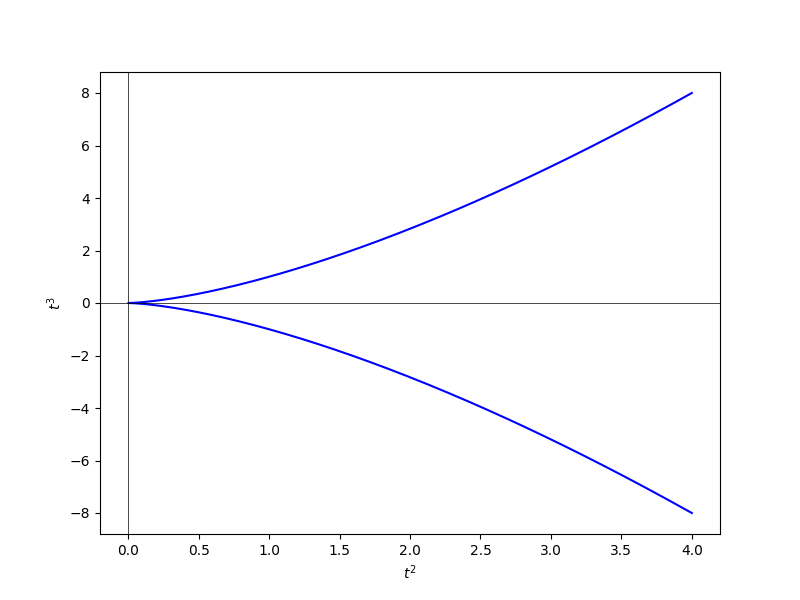
\includegraphics[width=0.5\textwidth]{fig1.png}
			\end{figure}
			
			It is clear that it is a morphism.

			To see if it is continuous first remember that affine space (and also projective space) is equipped with the Zariski topology, whose open sets are complements of algebraic sets (=sets of zeroes of polynomials). But $A=k[x]$ is principal so every algebraic set is the set of zeroes of one polynomial, basically because of this corollary of the Nullstellensatz:
\begin{coro}[[Hart] 1.4]
	There is a one-to-one inclusion-reversing correspondence between algebraic sets in $\mathbb{A}^{n} $ and radical ideals in $k[x_1,\ldots,x_n$ ] (i.e., ideals which are equal to their own radical), given by $Y\mapsto I(Y)$ and $\mathfrak{a}\mapsto Z(\mathfrak{a})$. Furthermore, an algebraic set is irreducible iff its ideal is a prime ideal.
\end{coro}

And $k$ is closed so every polynomial $n$ roots, so algebraic sets are just finite sets.

{\color{magenta}This was seemed relevant at some point…}

\begin{defn}
	The \textit{\textbf{(Krull) dimension}} of a ring $A$ is the supremum of all \textit{\textbf{heights}} of all prime ideals, i.e. the largest proper chain of prime ideals $\mathfrak{p}_0\subset \mathfrak{p}_1\subset\ldots\subset \mathfrak{p}$.
\end{defn}

\begin{thing7}{Proposition 1.7}\leavevmode
	If $Y$ is an affine algebraic set, then the dimension of $Y$ is equal to the dimension of its affine coordinate ring $A(Y)$.
\end{thing7}

			We only need to know that closed sets are finite points. This \href{https://math.stackexchange.com/questions/407693/polynomials-are-continuous-with-respect-to-the-zariski-topology}{means} that polynomials are continuous functions with respect to Zariski topology (because preimage of a closed set=finite set of points is closed because it is the root of $p-\alpha$). That makes $\varphi$ continuous.

			Being bicontinuous is the same as being a homeomorphism, which is equivalent to showing that $\varphi$ is open or closed (since we already noted it is bijective). But, finite sets of points are closed sets in the curve (because it is put in affine space---this is not true in general!).

			Finally we show that $\varphi$ is not an isomorphism. Yesterday with Victor we tried to write the inverse map, which should satisfy
\begin{align*}
	 (x,y)&=(\varphi^{-1}(x,y)^2,\varphi^{-1}(x,y)^3)\\
	\implies &\begin{cases}
		\varphi^{-1}(x,y)^2&=x=\frac{x^2}{x^3}=\frac{x^2}{y^2}=\left(\frac{x}{y}\right)^2 \\
		\varphi^{-1}(x,y)^3& =y=\frac{y^2}{y^3}=\frac{x^3}{y^3}=\left(\frac{x}{y}\right)^3
	\end{cases}
\end{align*}
so basically $\varphi^{-1}$ must be $(x,y)\mapsto \frac{x}{y}$ but this is not defined at $y=0$ so I thought well why don't you just put
			\[(x,y)\longmapsto\begin{cases}
				0\qquad &y=0 \\
				\frac{x}{y}\qquad &y\neq 0
			\end{cases}\]
			but then all $(x,0)$ will map to $(0,0)$ under $\varphi\circ \varphi^{-1}$. So what happens is that this map is not well-defined so it is not an isomorphism.

	\item The Frobenius morphism is in fact a ring homomorphism meaining it preserves multiplication and addition. Addition is more \href{https://en.wikipedia.org/wiki/Frobenius_endomorphism#Definition}{interesting}: since $p$ is prime, it divides the numerator and not the denominator of the binomial coefficient $\frac{p!}{k!(p-k)!}$, and this will make that number 0 unless $k=0,n$, which are the first final terms of the binomial expansion  $(a+b)^p$. Therefore we must only show that $\varphi$ has trivial kernel. Now since $k$ is a field, all elements are units, so none of them can actually satisfy $a^p=0$, making $\ker\varphi=0$.

	That $\varphi$ surjective \href{https://en.wikipedia.org/wiki/Perfect_field}{follows} from an equivalence of the field being algebraically closed and thus perfect.

	That $\varphi$ is continuous and bicontinuous follows from the same reasons as the previous question.

	To finish we check that the induced map on coordinates rings is not an isomorphism, since its inverse must be of the form $t\mapsto t^{\frac{1}{p}}$, which is not polynomial.

\end{enumerate}
\end{proof}

\section{$\mathbb{P}^n$ minus a hyperplane (Alex)}

\begin{manualexercise}{3.5}[Alex, Sept 17]
	By abuse of language, we will say that a variety \textit{\textbf{is affine}} it is isomorphic to an affine variety. If $H\subseteq \mathbb{P}^n$ is any hypersurface, show that $\mathbb{P}^n-H$ is affine.
\end{manualexercise}

\begin{proof}[Solution]\leavevmode
	Suppose $H=V(f)$ with  $\operatorname{deg}f=d$. Consider the $d$-uple embedding $v_d:\mathbb{P}^n\to \mathbb{P}^N$
\end{proof}

\section{Products of Quasi-Projective Varieties (extra)}

\begin{manualexercise}{3.16}[Products of Quasi-Projective Varieties]
	Use the Segre embedding (Ex. 2.14) to identify $\mathbb{P}^n\times\mathbb{P}^m$ with its image and hence give it a structure of projective variety. Now for any two quasi-projective varieties $X\subseteq\mathbb{P}^n$ and $Y\subseteq\mathbb{P}^m$ consider $X\times Y\subseteq\mathbb{P}^n\times\mathbb{P}^m$.
	\begin{enumerate}[label*=(\alph*)]
		\item Show that $X\times Y$ is a quasi-projective variety.
		\item If $X,Y$ are both projective, show that $X\times Y$ is projective.
		\item Show that $X\times Y$ is a product in the category of varieties.
	\end{enumerate}
\end{manualexercise}

\begin{proof}[Solution]
	content...
\end{proof}

\section{Normal varieties (Victor)}

\begin{manualexercise}{3.17}[Normal varieties]
	\end{manualexercise}

\begin{manualexercise}{3.18}[Projectively Normal Varieties]
\end{manualexercise}

	\begin{defn}\leavevmode 
		\begin{itemize}
		\item A variety $Y$ is \textit{\textbf{normal}} ar a point $P\in Y$ if $\mathcal{O}_{P}$ is an integrally closed ring. Y is \textit{\textbf{normal}} if it is normal at every point.
		\item A projective variety $Y\subseteq \mathbb{P}^n$ is \textit{\textbf{projectively normal}} (with respect to the given embedding) if its homogeneous coordinate ring $S(Y)$ is integrally closed.

		\item 	Let $A\subset B$ be a subring (or a morphism $A\to B$) $b\in B$ is \textit{\textbf{integrally closed}} if it is the root of a polynomial in $A[x]$. Here we mean that  $S(Y)$ equals the set of integrally closed elements with respect to its field of fractions.
\end{itemize}
	\end{defn}

	\begin{enumerate}[label=\alph*.]
		\item If $Y$ is projectively normal, then $Y$ is normal.

		\item There are normal varieties in projective space which are not projectively normal. For
	\end{enumerate}

\begin{proof}[Solution]\leavevmode
	\begin{enumerate}[label=\alph*.]
		\item $\forall p \in Y$ and prime ideal $\mathfrak{m}_p  \in\operatorname{Spec}(Y)$ we have
			\[S(Y)\subseteq S(Y)_{\mathfrak{m}_p}\subseteq F(Y)\]
			{\color{magenta}How does this conclude?}

		\item 
	\end{enumerate}
\end{proof}

\addcontentsline{toc}{section}{5.4}
\begin{manualexercise}{5.4}[Intersection mulitplicity]
	If $X,Y\subseteq \mathbb{A}^{2} $
\end{manualexercise}

\section{September 10}

\subsection{Analitycally isomorphic singularities (Arthur)}

\subsubsection{Arthur's notes}

\begin{thing5}{Exercise 5.14}\leavevmode
	
\end{thing5}

\begin{enumerate}[label=(\alph*)]
	\item
	\textbf{Problem:} Show that if two points of two plane curves are analytically isomorphic then they have the same multiplicity.
	
	Let $A = k[x,y]/(f)$ and $\mathfrak{m} = (x,y)A$. Then $A/\mathfrak{m}^n \simeq \hat{A}/\mathfrak{m}^n\hat{A}$ for all $n \geq 0$. Setting $r = \mu(f)$, we have $(f) \subseteq \mathfrak{m}^r$ and $(f) \subsetneq \mathfrak{m}^{r+1}$. Hence
	\begin{equation*}
		\dim \hat{A}/\mathfrak{m}^n\hat{A} = \dim A/\mathfrak{m}^n = \dim \frac{k[x,y]}{(x,y)^n} \quad \text{for all } n \leq r.
	\end{equation*}
	[Dimensions of $k$-vector spaces.]
	However
	\begin{equation*}
		\dim \hat{A}/\mathfrak{m}^{r+1}\hat{A} = \dim A/\mathfrak{m}^{r+1} = \dim \frac{k[x,y]}{(f)+(x,y)^{r+1}} < \dim \frac{k[x,y]}{(x,y)^{r+1}}.
	\end{equation*}
	Therefore we have a characterization of $r=\mu(f)$ as the first $n \geq 0$ such that $\dim \hat{A}/\mathfrak{m}^{n+1}\hat{A} \ne \dim k[x,y]/(x,y)^{n+1}$. Since this characterization depends only on the completion of $A$, we have obtained a solution to the the problem.
	
	\item Let $f,g \in k[[x,y]]$. Write $f = f_r + f_{r+1} + \cdots$,
	where the $f_d \in k[x,y]$ are homogeneous of degree $d$.
	Suppose
	\[ f_r = g_sh_t, \]
	where $g_s$ and $h_t$ homogeneous of degrees $s$ and $t$, and have no common linear factor.
	
	\textbf{Problem:} Find power series
	\begin{align*}
		g &= g_s + g_{s+1} + \cdots, \\
		h &= h_t + h_{t+1} + \cdots
	\end{align*}
	such that $f=gh$.
	
	Expand the product to find
	\begin{equation*}
		f = \sum_{d=0}^\infty \left( \sum_{i+j=d} g_{s+j}h_{t+i} \right).
	\end{equation*}
	Looking at homogeneous parts of degree $r+d$, we see that our problem is solved as soon as we have
	\begin{equation} \label{eq:frd}
		f_{r+d} = \sum_{i+j=d} g_{s+j}h_{t+i} = (g_{s+d}h_t + g_sh_{t+d}) + \sum_{\substack{i+j=d\\ i,j \ne 0}} g_{s+j}h_{t+i}.
	\end{equation}
	Hence, one way of solving the problem is to inductively find the polynomials $g_{s+d}, h_{t+d}$.
	
	Since $g_s$ and $h_t$ don't have linear factors in common in $k[x,y]$, the polynomials $g_s(t,1)$ and $h_t(t,1)$ don't have common linear factors in $k[t]$ and so generate they $k[t]$.
	Given a homogeneous $a(x,y) \in k[x,y]$, we can therefore find $p(t), q(t) \in k[t]$ such that
	\[ g_s(t,1)p(t) + h_t(t,1)q(t) = a(t,1). \]
	Taking $t = x/y$ and multiplying the expression above by $y^{\deg a}$, we obtain
	\[ g_s(x,y)\tilde{p}(x,y) + h_t(x,y)\tilde{q}(x,y) = a(x,y), \]
	where $\tilde{p}(x,y) = y^{\deg a -s}p(x/y), \tilde{q}(x,y) = y^{\deg a - t}q(x/y)  \in k[x,y]$ are homogeneous.
	
	In particular, we can find $g_{s+1}, h_{t+1} \in k[x,y]$ homogeneous such that
	\[ g_sh_{t+1} + g_{s+1}h_t = f_{r+1}; \]
	and homogeneous polynomials $g_{s+2}, h_{t+2}$ such that
	\[ g_sh_{t+2} + g_{s+2}h_t = f_{r+2} - g_{s+1}h_{s+1}. \]
	More generally, we can find $g_{s+i}, h_{t+i} \in k[x,y]$ such that
	\[ g_sh_{t+i} + g_{s+i}h_t = f_{r+i} - \sum_{\substack{i+j=d\\ i,j \ne 0}} g_{s+j}h_{t+i} \]
	
	Then equation \eqref{eq:frd} is satisfied and the problem is solved.
	
	%\textbf{Consequence:} The number of irreducible components of $\operatorname{Spec} \widehat{\oh_P}$ is equal to the number of distinct tangents of the curve at the origin (i.e., not counting multiplicities).
	
	\item Coming soon.
	
	\item Write $f(x,y) = f_2(x,y) + f_3(x,y) + \cdots + f_n(x,y)$.
	Using the change of coordinates $x \mapsto x+y$, we have that $f_2(x,y) = ay^2 + bxy + cx^2$ with $a \ne 0$.
	Then $f(x,y) = y^2 g(y)$ for some $g(y) \in k[y]$ such that $g(0) \ne 0$.
	
	The Weierstrass preparation theorem says that we may write
	\[ f(x,y) = U(x,y)(y^2 + a(x)y + b(x)) \]
	for \emph{unique} $U(x,y) \in k[[x,y]]$ and $a(x), b(x) \in k[[x]]$ such that $U$ is invertible and $a(0)=b(0)=0$. [We won't use this last condition.]
	Since $U$ is a unit,
	\[ \widehat{\mathcal{O}_P} \simeq \frac{k[[x,y]]}{(f(x,y))} = \frac{k[[x,y]]}{(y^2 + a(x)y + b(x))}, \]
	i.e., the curve is given near the origin by $y^2 + a(x)y + b(x) = 0$.
	
	Because $\operatorname{char} k \ne 2$, we can eliminate the linear term by completing the square and changing $y \mapsto y - a(x)/2$:
	\[ y^2 + a(x)y + b(x) = \left( y + \frac{a(x)}{2} \right)^2 - c(x) \]
	
	Now the equation is $y^2 - c(x) = 0$.
	But $c(x) = x^r V(x)$ for some $V(x) \in k[[x]]$ such that $V(0) \ne 0$.
	Since $\operatorname{char} k \ne 2$, we can then find a power series $U(x)$ such that $U(x)^2 = V(x)$. This is just solving the linear equations arising from
	\[ \sum a_nx^n = \left( \sum b_n x^n \right)^2 = \sum ( \sum_{\substack{i+j=n\\ i,j \ne n}} b_i b_j + b_0b_n ) x^n. \]
	
	Now we substitute $y \mapsto yU(x)$ to transform the ideal $(y^2 - x^rU(x)^2)$ into $(y^2 - x^r)$.
	
	Finally, uniqueness of $r$ follows from the uniqueness part of the Weierstrass preparation theorem:
	Given $f(x,y) \in k[x,y]$, we did $x \mapsto x + y$ and considered the polynomial $y^2 + a(x)y + b(x)$ given by the preparation theorem. There was no choice involved in these steps.
	After completing the square we saw that $r$ is the largest integer such that $x^r$ divides $c(x) = -b(x) + a(x)^2/4$; hence $r$ is uniquely determined by $f(x,y)$.
\end{enumerate}



\subsubsection{Notes from class}

Two curves $C_1,C_2$ with points $P \in C_1$ and $Q\in C_2$, and $\mathcal{O}_P\supset\mathfrak{m}_P$, $\mathcal{O}_Q\supset\mathfrak{m}_Q$. And
\[C:f=0,\qquad f[x,y]/(f), \quad \mathfrak{m}=(x,y).\]
We define
\[\hat{\mathcal{O}}_p=\lim_{\longleftarrow} \mathcal{O}_P/\mathfrak{m}^n_P\cong k[ [x,y]]/(y)\]

\begin{defn}
	\textit{\textbf{Analitical isomorphism}} is a $k$-isomorphism with $\hat{\mathcal{O}}_P\cong \hat{\mathcal{O}}_Q$.
\end{defn}

\begin{manualexercise}{}
	\begin{enumerate}[label=\alph*.]
		\item An. isomorphic $\implies \mu_{C_1}(D)=\mu_{C_2}(Q)$.
\[f(x,y)=f_r(x,y)+f_{r+1}(x,y)+\ldots+f_n(x,y).\]
\[\mu(p)=r\]

\item Let $f=f_r+f_{r+1}+\ldots\in k[[x,y]]$. Suppose that $f_r=g_s h_t\in k[x,y]$ have no linear factors in common (which means they are coprime). Then there exist $g,h\in k[ [ x,y] ]$ such that
	\[f=gh,\quad g=g_s,\quad h=h_t+\ldots\]

	\item Let $f=f_r+f_{r+1}+\ldots\in k[x,y]$. If
		\[f_r=L_1\cdot L_2\cdot \ldots\cdot L_r\]
		then $P=(0,0)$ is an ordinary $r$-fold. Show that any 2-folds are analitically isomorphic.

		\item Consider the curve $C:f=0,\quad \mu=2$. It is an ordinary 2-fold. Show that
			\[\hat{\mathcal{O}}_P\cong \frac{k[ [ x] ]}{(y^2-x^r)}\]
	\end{enumerate}
\end{manualexercise}

\begin{proof}[Solution]\leavevmode
	\begin{enumerate}[label=\alph*.]
		\item

		\item Suppose they exist and are $g=\sum_{i}g_i$, $h=\sum_{j}h_j$ so that
			\[f=gh=\sum_{d=r}^\infty\sum_{i+j=d}g_ih_j\]
			which means that
			\[f_{r+d}=\sum_{i+j=d}g_ih_j=g_sh_{t+d}+g_{s+d}h_t+\sum_{?}g_ih_j\]
			and
			\[f_{r+1}=g_s h_{t+1}+g_{s+1}h_t\]
			Notice that since $g$ and $h$ don't share linear factors, we may fix the second variable and the resulting polynomials generate $k[t]$, ie.
			\[(g_s(t,1),h_t(t,1))=k[t]\]
			Further computations show that the next term is well defined.

		\item Consider the completion at the origin, $\hat{\mathcal{O}}_P\cong k[[x,y]]/(f)$. We shall try to show that in fact
			\[k[[x,y]]/(f)\overset{\cong }{\longrightarrow}k[ [x,y]]/(f_r)\]
			so consider the map
			\begin{align*}
				x\mapsto x+A(x,y)\qquad \qquad y\mapsto y+B(x,y)
			\end{align*}
			so that
			\[f(x+A(x,y),y+B(x,y))=f_r(x,y).\]
			Using a projective transformation, that makes the tangents be (?), we see that
			\[\hat{\mathcal{O}}_P\cong k[ [x,y]]/(xy)\]

			\begin{claim}[Not true]
		 Any $k$-isomorphism 
		 \[\varphi:\frac{k[ [x,y]]}{(f)}\longrightarrow\frac{k [ [ x,y] ] }{(y)}\]
		 have the form
		 \[x\mapsto x+A(x,y)\quad \quad y\mapsto y+B(x,y)\quad  \text{when } \mu\geq 2\]

		 \item Suppose that
			 \[f(x,y)=y^2A(y)\qquad A(0)\neq 0,\qquad f(x,y)=(y^2+a(x)y+b(x))\cdot u(x,y)\]
			 recall that
			 \begin{thm}[Weierstrass preparation theorem]\leavevmode
				 Let $A$ be a local ring, $k[ [x]]$,  $\mathfrak{m}=(x)$, and $f\in A[ [ y ] ]$. Then
			 \[f=(y^n+k_{r-1}y^{n-1}+\ldots+b_0)\cdot u(y)\]
			 for $u\in A[ [ y] ]^\times $ and $b_i\in\mathfrak{m}$
			 \end{thm}
			 \begin{align*}
			 	f(x,y)& =(y^2+c(x))u(x,y)\\
				\hat{\mathcal{O}}_P&\cong \frac{k[ [x,y]]}{(y^2+c(x))}\\
				c(x)& =x^rV(x),\quad \text{where } V\in k[ [ x]]^\times \\
				V(x)& =1+x+\ldots\\
				\sqrt[r]{1+x} =1+c_1x+\ldots\\
				V(x)& =W(x)^r\\
				x^rV(a)& =(xW)^r\\
				y^2&-x^r.
			\end{align*}
	\end{claim}

	\end{enumerate}
\end{proof}

\subsection{Degree and Hilbert polynomial (Bruno)}

%\addcontentsline{toc}{subsubsection}{Exercise 7.2}

\begin{defn}
	Let $M=\bigoplus_{t}M_t$ be a finitely generated graded $S$-module, where $S=k[x_0,\ldots,x_m]$. A \textit{\textbf{Hilbert function}} is
	\begin{align*}
		\varphi: \mathbb{Z} &\longrightarrow M \\
		t &\longmapsto \dim_k(M_t)
	\end{align*}
\end{defn}

\begin{thm}[Definition]
	There exists a unique polynomial $P_M\in\mathbb{Q}[t]$ called the \textit{\textbf{Hilbert polynomial}} such that for all $t\gg 0$, $P_M(t)=\varphi_M(t)$.
\end{thm}

\begin{thing5}{Repetition}\leavevmode
	Let me put a quote from \href{https://en.wikipedia.org/wiki/Hilbert_series_and_Hilbert_polynomial#Definitions_and_main_properties}{wiki} so that I never forget what is the Hilbert polynomial:
	{\color{6}\begin{quotation}
			[…] This shows that there exist a unique polynomial $HP_X(n)$ with rational coefficients which is equal to $HF_S(n)$ for $n$ large enough. This polynomial is the \textit{\textbf{Hilbert polynomial}}, and has the form
			\[HP_S(n)=\frac{P(1)}{(\delta-1)}n^{\delta-1}+\text{ terms of lower degree in } n\]
	\end{quotation}}
\end{thing5}

\begin{manualexercise}{7.2}
	Let $Y$ be a variety of dimension $r$ in $\mathbb{P}^n$, with Hilbert polynomial $P_Y$. We define the \textit{\textbf{arithmetic genus}} of $Y$ to be
	\[P_Y(t):=P_{S[Y]}(t)\]
	\[=(-1)^r(P_Y(0)-1)\]
	\begin{enumerate}[label=\alph*.]
		\item  $Y=\mathbb{P}^n$.
		\item $Y\subset \mathbb{P}^n$ plane curve of degree $d$.
		\item $ Y\subset \mathbb{P}^n$ hypersurface of degree $d$.
		\item $Y_a,Y_b\subset \mathbb{P}^3$ of degrees $a$ and $b$, $Y =Y_a\cap Y_b$ complete intersection.
		\item $Y^r\subset \mathbb{P}^n$, $Z^s\subset \mathbb{P}^m$ : $Y\times Z\subset \mathbb{P}^N$. Here
			\[P_{Y\times Z}(t)=P_Y(t)P_Z(t)\]
	\end{enumerate}
\end{manualexercise}

\begin{proof}[Solution]\leavevmode
	\begin{enumerate}[label=\alph*.]
		\item $S[Y]=k[x_0,\ldots,x_n]$, 
		\[\dim (k[x_0,\ldots,x_n]_t)=\binom{n+t}{n}=\frac{(n+1)(n+t-1)\ldots(t+1)}{n!}=\frac{t^n}{n!}+\ldots\]
			so that
			\[P_Y(0)_1\implies P_a(\mathbb{P}^n)=0.\]
	
			\item Now
				\[P_a(Y)=\frac{(d-1)(d-2)}{2}\]
				which follows from c so let's do c.

			\item Suppose $Y=Z(f)$. Then
			\[(f)\hookrightarrow k[x_0,\ldots,x_n]\to k[Y]\]
			\begin{align*}
				(f)& =\{f\varphi:\varphi\in k[x_0,\ldots,x_n]\} \\
				(f)_t&=\binom{n+t-d}{n}\\
			P_Y(t)&=\binom{n+t}{n}-\binom{n+t-d}{n}\\
			P_a(Y)&=(-1)^n\binom{n-d}{n}\\
			&=(-1)^n\frac{(n-d)(n-d-1)\ldots(1-d)}{n!}\\
			&=\frac{(d-1)\ldots(d-n)}{n!}\\
			& =\binom{d-1}{n}
			\end{align*}

			\item Let's first write the formula and then we discuss it
				\begin{align*}P(t)&=\binom{3+t}{t}-\binom{3+t-a}{t}-\binom{3+t-b}{t}+\binom{3+t-a-b}{3}\\
					&=(ab)t+P_Y(0)
					\end{align*}
					\begin{align*}
						P_Y(0)&=1-f(a)-f(b)+f(a+b)\\
						P_a(Y)&=f(a)+f(b)-f(a+b)
					\end{align*}
					Considering multiplication by $f_b$ as map
					\[\frac{k[\mathbb{P}^3]}{(f_a)}\overset{f_b}{\longrightarrow}\frac{k[\mathbb{P}^3]}{(f_a)}\]
					so we get
					\[\begin{tikzcd}
						0\arrow[r]&\frac{k[\mathbb{P}^3]}{(f_a)}\arrow[r]&\frac{k[\mathbb{P}^3]}{(f_a)}\arrow[r]&\frac{k[\mathbb{P}^3]}{(f_a,f_b)}\arrow[r]&0
					\end{tikzcd}\]
					but we need to consider the map $[-b]$ to stop the grading from moving up from one arrow to another. Then we get
					\[P_Y=P_{Y_a}(t)-P_{Y_a}(t-b)\]
					so
					\[P_A-P_B+P_C=0.\]

	\item O problema est\'a em ver se
		\[K[Y\times Z]_d\overset{?}{\cong}k[Y]_d \otimes_k k[Z]_d\]
	Da\'i o Hilbert polynomial \'e o produto dos Hilbert polynomials e t\'a.
	\end{enumerate}
\end{proof}

\section{September 13}

\subsection{Veronesse surface (Alex)}

\begin{manualexercise}{2.13}
	Let $Y$ be the image of the 2-uple embedding of $\mathbb{P}^2$ in $\mathbb{P}^{5}$. This is the \textit{\textbf{Vernoses surface}}. If $Z\subseteq Y$ is a closed curve (a \textit{\textbf{curve}} is a variety of dimension 1), show that there exists a hypersurface $V\subseteq \mathbb{P}^5$ such that $V \cap Y=Z$.
\end{manualexercise}

\begin{proof}[Solution]\leavevmode
	\begin{align*}
		\rho_2: \mathbb{P}^2 &\overset{\text{Veronese} }{\longrightarrow}\mathbb{P}^5\\
		[x_0:x_1:x_2]&\longmapsto [x_0^2:x_1^2:x_2^2:x_0x_1:x_1x_2:x_0x_2]
	\end{align*}
	And $Y:=\rho_2(\mathbb{P}^2)$. Notice that $Y=\mathbb{V}(\ker \theta)$ where
	\begin{align*}
		\theta: k[y_0,\ldots,y_5 &\longrightarrow k[x_0,\ldots,x_2] \\
		y_i &\longmapsto M_i=\text{$i$-th monomial of degree $d$ in $x_0,\ldots,x_n$}\\ \\
		y_0&\longmapsto x_0^2\\
		y_1&\longmapsto x_1^2\\
		y_2&\longmapsto x_2^2\\
		y_3&\longmapsto x_0x_1\\
		y_4&\longmapsto x_0x_2\\
		y_5&\longmapsto x_1x_2
	\end{align*}
 it is not immediate that kernel of this map is $Y$, but it is true.

 By exercise 2.8 there exists a homogeneous polynomial (which is irreducible) such that $V(f)=\rho^{-1}_2(Z)$. Recall that $Z$ is a curve in $Y$ so $\rho^{-1}(Z)$ is (probably) a curve in $\mathbb{P}^2$.

 So, we have
 \[Z=\rho_2(V(f))=\rho_2(V(f^2)),\]
 which follows from the fact that $\theta$ is surjective over the set of polynomials of even degree. How to prove this? It sufficies to prove for monomials. This is a combinatorial problem. Consider
 \[x_0^{a_0}x_1^{a_1}x_2^{a_2}\longmapsto(a_0,a_1,a_2)\in\mathbb{Z}^3\]
 Anyway… this means that there exists $g\in k[x_0,x_1,x_2]$ such that $f^2=\theta(g)$. And then
 \[Z=Y\cap V(g)\]
 which means that being the Veronese image of a zero of $f$ is the same as being a zero of $g$. (Some more thought on how $\theta$ is working?)
\end{proof}

\paragraph{Explanation} The Veronese map image is actually the symmetric matrices of rank 1:
\begin{align*}
	v&\longmapsto v^{\mathbf{T}}\cdot v\\
	\begin{pmatrix} v_0\\v_1\\v_2 \end{pmatrix} \begin{pmatrix} v_0&v_1&v_2 \end{pmatrix} & =\begin{pmatrix} v_0v_0&v_0v_1\\v_1v_0&v_1v_1 \end{pmatrix} 
\end{align*}

\subsection{Degree of Veronese and Segre embeddings (Alex)}

%\addcontentsline{toc}{subsection}{Exercise 7.1}
\begin{manualexercise}{7.1}\leavevmode 
	\begin{enumerate}[label=\alph*.]
		\item Find the degree of the 2-uple embedding of $\mathbb{P}^n$ in $\mathbb{P}^N$.

		\item Find the degree of the Segre embedding of $\mathbb{P}^r\times \mathbb{P}^s$ in $\mathbb{P}^N$.
	\end{enumerate}
\end{manualexercise}

\begin{proof}[Solution]\leavevmode
\begin{enumerate}[label=\alph*.]
	\item Recall that the degree of a map the coefficient of greatest degree of the Hilbert polynomial times the degree factorial, i.e. if the Hilbert polynomial is
	\[P_{X}(z)=a_nz^n+\ldots+a_0,\]
	the degree of $X$ is
	\[a_nn!\]
	(So remember that the Hilbert polynomial is the unique polynomial in $\mathbb{Q}[t]$ that equals the Hilbert function (the Hilbert functions at $n$ is just the dimension of the degree-$n$ component of $S[X]=\bigoplus_{n} S_n $, so homogeneous polynomials of degree $n$) for sufficiently large numbers.)

	\begin{claim}
		\[S(X)_m \cong k[x_0,\ldots,x_n]_{md}\]
		where $d$ is the $d$ in the $d$-uple embedding.
	\end{claim}
	If we show this, we can see that
	\[P_{x}(m)=\binom{md+n}{n}=\prod_{i=1}^n\frac{(md+i)?}{n!}=\frac{d^nm^n}{n!}+\text{lower order terms}  \]
	Now the pullback map is
	\[\frac{k[x_0,x_1,\ldots,x_N}{I(X)}\overset{\cong }{\longrightarrow}?k[x_0,x_1,\ldots,x_n]\]

	\item 
	
	\end{enumerate}

\end{proof}


\subsection{Curvas elípticas (Carlos)}

$k$ n\~ao neces. algebricamente fechado, $\bar{k}$ algebraic closure, $V$ variedade afim, $V\subseteq \mathbb{A}^n=k^n$, $k[V]=k[c_1,\ldots,x_n]/I(V)$. $P\in V$, $\mathfrak{m}_p=\{g\in k[V]:g(p)=0\}$ \'e um ideal maximal.

Para $g\in k[V]$,
\[\operatorname{ord}_P(g)=\operatorname{sup}\{d\in\mathbb{Z}_{\geq 0}:g\in\mathfrak{m}_p^d\}.\]
Uma \textit{\textbf{curva}} \'e uma variedade projetiva suave de dimens\~ao 1. \textit{\textbf{Curvas el\'ipticas}}:
\[\begin{tikzcd}
	E:x^2=x^3+ax+b\arrow[d,"\text{projetiza\c c\~ao}" ]\\
	zy^2=x^3+axz^2+bz^3
\end{tikzcd}\]

\begin{exercise}
	Seja $E/k$ uma curva eliptica suave:
	\begin{align*}
		y^2&=x^3+ax+b\\
		&=(x-e_1)(x-e_2)(x-e_3)
	\end{align*}
	com $e_1,e_2,e_3\in\bar{k}$. Considere
	\[f_1=(x-e_1),\quad f_2=(x-e_2),\quad f_3=(x-e_3)\]
	\[p_1=(e_1,0),\quad p_2=(e_2,0),\quad p_3=(e_3,0)\]
	O que \'e
	\[\operatorname{ord}_{f_i}p_i=?\]
\end{exercise}

\begin{proof}[Solution] Lembre que $p$ \'e um ponto suave se e somente se $\dim \mathfrak{m}_p/\mathfrak{m}_p^\alpha=\dim V$.
	\begin{enumerate}[label=\textbf{Step \arabic*}]
		\item Considere a projetiza\c c\~ao de $E$ :
			\[y^2z=(x-e_1z)(x-e_2z)(x-e_3z).\]
			Da\'i,
			\[p_1=[e_1:0:1],\quad p_2=[e_2:0:1],\quad p_3=[e_3:0:1]\]
			
	\end{enumerate}
\end{proof}

\section{September 17}
\subsection{Dimension of affine variety $\cap$ hyperplane (Alex+Arthur)}

\begin{manualexercise}{1.8}
	Let $Y$ be an affine variety of dimension $r$ in $\mathbb{A}^n$. Let $H$ be a hypersurface in $\mathbb{A}^n$ and assume that $ Y\not\subseteq H$. Then every irreducible component of $Y\cap H$ has dimension $r-1$.

	So: intersection of variety of dimension $r$ and hypersurface is variety dimensin $r-1$.
\end{manualexercise}

\begin{proof}[Solution]\leavevmode
	Suppose $H=\mathbb{V}(f)$ and $Y=\mathbb{V}(\mathfrak{q})$. Then $Y\cap H=\mathbb{V}(\mathfrak{q}+(f))$. Pick an irreducible component in $Y\cap H$ which is associated to a prime ideal $\mathfrak{p}$. Then we have that $\mathfrak{q}+(f)\subseteq \mathfrak{p}$. Passing to the quotient, we have that $(f)/\mathfrak{q}\subseteq \mathfrak{p}/\mathfrak{q}$. Now we use the result that

	\begin{thm}[Krull's Hauptidealsatz]
		Let $A$ be a noetherian ring. For an element $x\in A$ that is not a unit nor a zero divisor,
		\[(x)\subseteq \mathfrak{p},\]
		where $\mathfrak{p}$ is a minimal ideal, then $\mathfrak{p}$ has height 1.
	\end{thm}
and since $(f)/\mathfrak{q}$ is principal in the quotient, ie. $(f)/\mathfrak{q}=(f+\operatorname{mod}\mathfrak{q})$.
\end{proof}


\section{Sept 20}
\subsection{Scroll (Sergey)}

You can find this $\operatorname{Sec}^k$ on a book by Harris, name?

There is an exercise from last class:
%\addcontentsline{toc}{subsubsubsection}{Exercise from Sergey, Sept 17}
\begin{manualexercise}{from Sergey, Sept 17}
	Compute $\operatorname{Sec}^k $ of $\operatorname{Segre}(a,b)$.
\end{manualexercise}

For today:
%\addcontentsline{toc}{subsubsubsection}{Exercise}
\begin{manualexercise}{(Sergey, Sept 20)}\leavevmode 
	\begin{enumerate}[label=\alph*.]
		\item Compute $\dim \operatorname{Gr}(k,N)$. You can use that $\operatorname{GL}(N)$ acts transitively.
		\item $\dim \operatorname{Sec}^k\operatorname{Gr}(N,2)$. \textbf{Hint:} Use linear algebra: $\Sigma_{0,n}=\operatorname{Cone}(\mathcal{v}_{n}\mathbb{P}^1$, $\mathbb{F}_{n}$ Hinzbruch surfaces. Rational Ruled Normal Surfaces (see below for definition of scroll ie. $\Sigma_{0,n}$.
	\end{enumerate}
\end{manualexercise}

\begin{proof}[Solution (Victor, September 27)]\leavevmode
	\begin{enumerate}[label=\alph*.]
		\item Consideremos os pontos da Grassmaniana $\operatorname{Gr}(m,N)$ como classes de equivalência de bases de vetores identificadas baixo a ação de $\operatorname{GL}(n)$. Considere uma base $(v_1,\ldots,v_m)$. Ela pode ser pensada como uma matriz de $N\times m$ de rango maximo, ie. ela tem posto $m$. Então, essa matriz tem uma submatriz de $m\times m$ não singular, e uma submatriz de $m(N-m)$ que  é singular. Variando as entradas dessa matriz singular, obtemos coordenadas para uma variedade de  dimensão $m(N-m)$. {\color{4}[Explicar mais]}

\begin{defn}[Extra: mergulho de Pl\"ucker, Sept 27]
	A Grassmaniana é uma variedade projetiva:
	\begin{align*}
		P_k: \operatorname{Gr}(m,V) &\longrightarrow \mathbb{P}\left( \Lambda^m(V) \right)  \\
		W &\longmapsto [w_1\wedge \ldots \wedge w_n]
	\end{align*}
	onde $W$  está generado por $w_1,\ldots,w_n$. Aqui tem que mostrar que isso está bem definido.
\end{defn}

\item Lembre que
	\begin{defn}
		(Ver  \href{https://en.wikipedia.org/wiki/Secant_variety}{Wiki}) Dada uma variedade projetiva $V\subset \mathbb{P}^r$, \textit{\textbf{variedade secante}} de $V$ é
		\[\operatorname{Sec}^k(V)=\overline{\{\overline{x_1,\ldots,x_k}:x_1,\ldots,x_k\in V\}}\]
		Em palavras, o fecho de Zariski do conjunto de "espaços generados" por $k$-tuplas de pontos em $V$. Por exemplo,
		\[\operatorname{Sec}^2(V)=\overline{\{\overline{xy}:x,y\in V\}}\]
		é o fecho de Zariski do conjunto de todas as linhas secantes a $V$ em $\mathbb{P}^r$. Mais geralmente, a \textit{\textbf{$k$-ésima variedade secante}} é o fecho de Zariski da união de todos os espaços lineares generados por coleções  de $k$ (ou $k+1$?) pontos em  $V$. (Note que os espaços lineares numa variedade projetiva são as projetivizações dos espaços lineares correspondentes no espaço afim.)
	\end{defn}
Pegue dois elementos em $\operatorname{Gr}(2,N)$, digamos $W,W'$ e pegue bases delas  $\{w_1,w_2\}$ e $\{w_1',w_2'\}$. Daí considere
\begin{align*}
	 \left\{ \big(tw_1-(1-t)w_1', tw_2-(1-t)w_2'\big)\right\}
\end{align*}

	\end{enumerate}
\end{proof}

\begin{defn}
	The \textit{\textbf{Segre embedding }} is 
	 \begin{align*}
		 \mathbb{P}(U)\times \mathbb{P}(V)&\hookrightarrow \mathbb{P}(U\otimes W)  \\
		 ([u],[v]) &\longmapsto [u\otimes v]
	\end{align*}
	Now take $X\subset \mathbb{P}(W)$. Then
	\[\operatorname{Sec}^k(X)=\overline{Z}\]
	where
	\[Z=\{[w]:\exists p_1,\ldots,p_k\in X\hookrightarrow \mathbb{P}(W)\} =\bigcup_{p_1,\ldots,p_k\in X}\left<p_1,\ldots,p_k\right>  \]
	where $p_i=[v_i]$ and $w=\sum_{i}v_i$.
\end{defn}

\begin{defn}[Scroll]
	I have a variety $X$ and two linear systems:
	\[\begin{tikzcd}
	&X\arrow[dl,"\varphi",hook,swap]\arrow[dr,"\psi",hook]\\
	\mathbb{P}(U)&&\mathbb{P}(V)
	\end{tikzcd}\]
	Then the \textit{\textbf{scroll}} is
	\[\mathbb{P}(U\oplus V)\supset\Sigma_{\varphi,\psi}=\{[u\oplus v]:[u]\in\varphi(X),[v]\in\psi(X)\}\]
	\textbf{Exercise:} Show this is a projective variety.

	So the scroll is a union of projective lines. It is called scroll because lines in one direction survive (in a drawing, they are all parallel) but the other lines are curved (so it looks like a scroll).
\end{defn}

%\addcontentsline{toc}{subsubsubsection}{Exercise about scroll}
\begin{manualexercise}{about scroll}
	As abstract varieties, $\Sigma_{a,b}$ is isomorphic to $\Sigma_{a'b'}$ iff $b-a=b'-b'=n$ and either  $a=a'=0$ or  $a>0, a'>0$.
\end{manualexercise}

\subsection{Elliptic curve is not rational (Alex)}
%\addcontentsline{toc}{subsubsubsection}{Exercise 6.3, Elliptic curve is not rational}
\begin{manualexercise}{6.3, Elliptic curve is not rational}
	Let  $Y$ be the curve $y^2=x^3-x$ in $\mathbb{A}^2$, and assume that the characteristic of the base field $k$ is not 2. In this exercise we will show that $Y$ is not a rational curve, and hence $K(Y)$ is not a pure trascendental extension of $k$.
\begin{enumerate}[label=\alph*.]
	\item Show that $Y$ is nonsingular, and deduce that $A=A(Y)\cong \frac{k[x,y]}{(y^2-x^3+x}$.
	\item Let $k[x]$ be the subring of …
\end{enumerate}
\end{manualexercise}

%\addcontentsline{toc}{subsubsection}{Exercise 6.2}
\begin{manualexercise}{6.2}
Let
	\[Y=V(y^2-x^3+x\subset \mathbb{A}^2\]
	be an elliptic curve. Show it is not rational.
\end{manualexercise}

\begin{defn}
	A curve $C$ is \textit{\textbf{rational}} if $C$ is birationally equivalent to $\mathbb{P}^1$
\end{defn}

\paragraph{Fact} If $C$ is a nonsingular rational but not isomorphic to $\mathbb{P}^1$, then $A(C)$ is a UFD.

\begin{enumerate}[label=\textbf{Step \arabic*}]
	\item $Y$ is nonsingular. Looks like we can just differentiate here and find that the zero locus of the derivatives is not in $C$.
\begin{defn}[Tangent space]
	Consider the local ring at the point and its maximal ideal. So $\mathfrak{m}_{p}/\mathfrak{m}^2_p$ is the \textit{\textbf{cotangent space}}. Then the  \textit{\textbf{tangent space}} is the dual  $\left(\frac{\mathfrak{m}}{\mathfrak{m}^2}\right)^*$. A point is \textit{\textbf{singular}} if the tangent space has more dimension than it should.
\end{defn}

\paragraph{Interpretation} Functions in $\mathfrak{m}_p$ are those which vanish at $p$. A function in $\mathfrak{m}^2_{p}$ is $\sum_{i}f_ig_i$ so its differential is $ d \left( \sum_{i}f_ig_i \right) =\sum_{i}f_idg_i+\sum_{i}g_ifd_i$ which you want to mod out because it is zero at $p$ because both $f_{i}$ and $g_{i}$.

\begin{remark}
	For $X,Y\subset Z$, $T_pX,T_pY\subset T_pZ$
	\[T_p(X\cap Y)=T_pX\cap T_pY\]
\end{remark}

\item 
	\begin{thing6}{Theorem 5.1}\leavevmode
		$Y\subseteq \mathbb{A}^n$ affine variety and $P\in Y$. Then $Y$ is nonsingular at $P \iff $ local ring $\mathcal{O}_{P,Y}$ is a regular local ring
	\end{thing6}
	\begin{thing6}{Theorem 6.2A}\leavevmode
		$A$ noetherian local domain of sdimension one with maximal ideal $\mathfrak{m}$. Then the following are equivalent
		\begin{enumerate}[label=(\roman*)]
			\item $A$ is a regular local ring.
			\item $A$ is integrally closed (over the fraction field).
		\end{enumerate}
	\end{thing6}
	In other words, normality in dimension 1 is the same as normality.

	\item Here's the \textit{\textbf{hyperelliptic involution}}
		\begin{align*}
			\sigma: k[Y] &\longrightarrow K[Y] \\
		x &\longmapsto x\\
		y&\longmapsto-y
	\end{align*}
	and then there's the \textit{\textbf{norm}}
	\begin{align*}
		N: K[Y] &\longrightarrow K[Y] \\
		a&\longmapsto a\sigma(a)
	\end{align*}
	Notice that
	\[N(1)=1\qquad N(a,b)=N(a)N(b)\]
	\textbf{Explanation:} we are killing $y$, so the norm takes us to a simpler space which is $Y/\sigma$.

This means $X$ is irreducible, $Y$ is irreducible. Then a discussion on the invertibility of the norm, units on these rings…
\end{enumerate}

 \subsection{Tangent map (Bruno)}

\begin{manualexercise}{5.10}
$X$ afine variety and $p\in X$.
\begin{enumerate}[label=\alph*.]
	\item $\dim T_pX\geq \dim X$, $\dim T_pX\iff p$ is nonsingular. Here $\dim X=\dim \mathcal{O}_{P,X}$ which is just the Krull dimension, so maximum height of chain of prime ideals.
	\item Define the tangent map.

	\item Project the parabola $x=y^2$ in $\mathbb{A}^2$ to the  $x$ axis and compute its derivative at 0.
		\end{enumerate}
\end{manualexercise}

\begin{proof}[Solution]\leavevmode
\begin{itemize}
\item $\dim T_pX=\dim \mathfrak{m}_p/\mathfrak{m}^2_p$, \textit{ as a vector space!} . Now that inequality is a result in homological algebra:
	\begin{thm}
		$A$ noetherian local domain and $ \mathfrak{m}$ maximal ideal then the dimension of the quotient of ideals as a vector space is greater or equal to the dimension of $A$ as a ring.
	\end{thm}
	\item 
		\begin{defn}
			$X\overset{\varphi}{\longrightarrow}Y$, $\varphi^*:\mathcal{O}_Y\to \mathcal{O}_X$ which is precomposition. Then since $\varphi(p)=q$ we see that $\varphi^*(\mathfrak{m}_q)\subset \mathfrak{m}_p\implies \varphi^* (\mathfrak{m}^k_q)\subset \mathfrak{m}^k_{p}$. And then take quotient by $\mathfrak{m}_{p}$ and $\mathfrak{m}^2_{q}$. These local rings are the functions that vanish at the point. Also they are localization of polynomials by maximal ideal.
		\end{defn}
\item
	 \begin{claim}
		 $(T\varphi)_0=0$
	\end{claim}
	look at the pullback
	\begin{align*}
		\varphi^*: k[\mathbb{A}^1] &\longrightarrow k[Z]=k[x,y]/(x-y^2) \\
		t &\longmapsto x
	\end{align*}
	which follows from definition.
	
	Then
	\[\varphi^*(\mathfrak{m}_{0})\subset \mathfrak{m}^2_{(0,0)}\implies \varphi^* :\mathfrak{m}_0/\mathfrak{m}_0^2\to \mathfrak{m}_{0,0}/\mathfrak{m}_{0,0}^2\]
	is zero because
	\[\varphi^* (t)=x=y^2,\qquad y\in\mathfrak{m}_{(0,0)}\]
	
\end{itemize}\end{proof}




%\addcontentsline{toc}{subsection}{Exercise Sergey}
\begin{manualexercise}{Sergey}
	Is the variety $\sum_{i=0}^sx_i^3=0$ rational in $\mathbb{P}^5$.
\end{manualexercise}

%\subsection{Blowing up curve singularities (Dani)}



\iffalse
\section{[Ot] Chapter I: Varieties}

A friend from Cabo Frio just recommended me to have a look at \href{https://www.uio.no/studier/emner/matnat/math/MAT4215/data/masteragbook.pdf}{Ottem\&Ellinsburg, Introduction to Schemes}. Here are some exercises I liked from Chapter 1: Varieties.

\addcontentsline{toc}{subsection}{Exercise 1.5.12}
\begin{manualexercise}{1.5.12}[The diagonal]
	Let $X$ be an affine variety and consider the map
	\begin{align*}
		\Delta: X &\longrightarrow X\times X \\
		x &\longmapsto (x,x)
	\end{align*}
	\begin{enumerate}[label=\alph*.]
		\item Show that $\Delta$ is a polynomial map.
		\item Let $X=\mathbb{A}^{n}(k)$…
		\item …gives an isomorphism $X\to \Delta(X)$. Hint…
	\end{enumerate}
\end{manualexercise}

\addcontentsline{toc}{subsection}{Exercise 1.5.15}
\begin{manualexercise}{1.5.15}
{\color{magenta}Some Lie groups that are algebraic sets}
\end{manualexercise}

\addcontentsline{toc}{subsection}{Exercise 1.5.28}
\begin{manualexercise}{1.5.28}
	Show that the image of the map
	\begin{align*}
		\phi: \mathbb{A}^{1}(k) &\longrightarrow \mathbb{A}^{3}(k) \\
		t &\longmapsto (t^{2},t^{3},t^{6})
	\end{align*}
	is given by $V(x^{3}-y^{2},z-x^{3})$. Show that $\phi$ is bijective. Is $\phi$ an isomorphism of affine varieties.
\end{manualexercise}

\addcontentsline{toc}{subsection}{Exercise 1.5.29}
\begin{manualexercise}{1.5.29}
	Show that the image of the map
	\begin{align*}
		\phi: \mathbb{A}^{1}(k) &\longrightarrow \mathbb{A}^{3}(k) \\
		t &\longmapsto (t^{3},t^{4},t^{5})
	\end{align*}
	is given by $V(x^{4}-y^{3},z^{3}-x^{5},y^{5}-z^{4})$. Show that $\phi$ is bijective. Is $\phi$ an isomorphism of affine varieties.
\end{manualexercise}

\addcontentsline{toc}{subsection}{Exercise 1.5.31}
\begin{manualexercise}{1.5.31}
	Show that the image of the map
	\begin{align*}
		\phi: \mathbb{P}^{1}(k) &\longrightarrow \mathbb{P}^{2}(k) \\
		(x_0:x_1( &\longmapsto (x_0^{2},x_0x_1,x_1^{2})
	\end{align*}
	is given by $V(y_1^{2}-y_0y_2)$. Show that $\phi$ is an isomorphism of projective varieties. Deduce that any projective conic is isomorphic to $\mathbb{P}^{1}(k)$.
\end{manualexercise}
\fi

\chapter{Chapter II}

\section{September 27}

\section{Sheaves (Bruno)}

\subsection{Background}
Let $X$ be a topological space and $\mathcal{F}$ a sheaf of rings, which is a presheaf + gluing condition.

\begin{thing2}{Sheafification}\leavevmode
	 \begin{align*}
	 	\text{Presheaf}  &\longrightarrow \text{Sheaf}  \\
	 	\mathcal{F} &\longmapsto \mathcal{F}^+
	 \end{align*}
 This $\mathcal{F}^+$ has two properties:
 \begin{enumerate}
 	\item Universal
		\[\begin{tikzcd}
			\mathcal{F}\arrow[r]\arrow[d]& G\\
		\mathcal{F}^+\arrow[ur]
		\end{tikzcd}\]
		
 \item For any $p\in X$, the stalks $\mathcal{F}_{p}=\mathcal{F}_{p}^+$.
 \item (Extra)
	 \[\begin{tikzcd}
	 	\text{Sheafs}\arrow[r,"\text{forget}" ]&\text{Presheaf}\arrow[l,bend left,"\text{Sheafify}" ]  
	 \end{tikzcd}\]
 \end{enumerate}
\end{thing2}
	 \begin{remark}
	 Also kernel and image of sheafs. Must sheafify the image.	
	 \end{remark}
	 
\subsection{Exercise 1.8}
Let $U\subset X$ be an open subset of $X$. Consider
\begin{align*}
	\Gamma(U,\cdot): \operatorname{Sheafs} &\longrightarrow \operatorname{Rings} \\
	\mathcal{F} &\longmapsto \Gamma(U,\mathcal{F})
\end{align*}
Show that $\Gamma(U,\cdot)$ is a left exact functor, that is,
\[\begin{tikzcd}
	0\arrow[r]&\mathcal{A}\arrow[r,"a"]&\mathcal{B}\arrow[r,"b"]&\mathcal{B}
\end{tikzcd}\]
exact implies
\[\begin{tikzcd}
	0\arrow[r]&\Gamma(U,\mathcal{A})\arrow[r,"a_U"]&\Gamma(U,\mathcal{B})\arrow[r,"b_U"]&\Gamma(U,C)
\end{tikzcd}\]

 %\end{enumerate}

 \begin{proof}[Solution]\leavevmode
 	\begin{itemize}
 	\item $a_V$ is injective is clear.
	\item $ \operatorname{img}a_U=\ker b_U$. Suppose $s \in\Gamma(U,\mathcal{B})$, so that $s =$
 	\end{itemize}
 \end{proof}

\section{September 24}

\subsection{Generically finite morphisms (Arthur)}

\begin{manualexercise}{3.7}
	
\end{manualexercise}

\begin{proof}[Solution]\leavevmode
	\textbf{First part.}
We will show the hint: the field extension $K(X) \subseteq K(Y)$ is finite.

Let $V = \operatorname{Spec} A \subseteq Y$ and $U = \operatorname{Spec} B \subseteq f^{-1}(V) \subseteq X$ be affine open subsets.
Write $C$ for the coordinate ring of $f^{-1}(\eta) \cap U$.

Since $f$ is of finite type, $C$ is finitely generated as a $K(Y)$-algebra.
Explain more. % B is fin gen over A and C is a quotient and localization of B
By Noether's normalization lemma, there exist $y_1, \ldots, y_d \in C$ such that $C$ is finite over $K(Y)[y_1,\ldots,y_d]$, where $d = \dim C$.
But $\dim C = \dim (f^{-1}(\eta) \cap U) = 0$ because $f^{-1}(\eta) \cap U$ is a finite set.
Hence $C$ is finite over $K(Y)$, i.e., $C$ is a finite $K(Y)$-vector space.
In particular, $K(X) \subseteq C$ is finite over $K(Y)$.

\textbf{Second part.}
We will show that there is an open affine $V \subseteq Y$ and an affine open cover $\{U_i\}$ of $f^{-1}(V)$ such that each restriction $U_i \to V$ is finite.

Let $V=\operatorname{Spec} A \subseteq Y$ be an open affine.
Since $f$ is of finite type, there is a finite affine open cover $U_i = \operatorname{Spec} B_i$ of $f^{-1}(V)$ such that $B_i$ is an $A$-algebra of finite type. Let $\{x_{ij}\}$ be a set of generators for $B_i$.
Now $B_i \subseteq K(X)$ and $K(X)$ is a finite $K(Y)$-module, so each $x_{ij}$ is integral over $K(Y)$, i.e., there are polynomials $P_{ij}(T) \in K(Y)[T]$ such that $P_{ij}(x_{ij}) = 0$.

There a is distinguished open subset $V_g \subseteq V$ such that $P_{ij}(T) \in \mathcal{O}_Y(V')[T]$ for all $i,j$.
Replace $U_i$ by $(U_i)_g$ and $V$ by $V_g$. Then $B_i$ is finite over $A$ because it is finitely generated by integral elements.
Hence $f : U_i \to V$ is a finite morphism ($U_i$ and $V$ are affine) for all $i$.

\textbf{Third part.}
Find an affine $V \subseteq Y$ such that $f^{-1}(V)$ is affine.

Now let $U \subseteq \bigcap_i U_i$ be an affine open.
Then $U \subseteq f^{-1}(V)$ and $f : U \to V$ is affine. We will show that we can choose an affine open $V' \subseteq V$ such that $f^{-1}(V') \subset U$. Then we will have $f : f^{-1}(V') \to V'$ affine, concluding the exercise.

To do this, let $Z = f^{-1}(V) \setminus U$.
If $\eta \in \overline{f(Z)}$ then actually $\eta \in f(Z)$ because it is the generic point of $V$.
Looking at the affine $U_i = \operatorname{Spec} B_i$, we see that any $z \in U_i \cap Z$ such that $\eta = f(z)$ corresponds to a prime $\mathfrak{p} \subseteq B_i$ such that $\mathfrak{p} \cap A = (0)$. Since $\mathfrak{p}$ is above the prime $(0) \subseteq A$, the following theorem tells us that $\mathfrak{p} = (0)$:

\begin{thm}[Cohen]\leavevmode
	
\end{thm}

But $(0) \in U$ and $Z \cap U = \varnothing$. Hence $\eta \not \in \overline{f(Z)}$.
Therefore there is some neighborhood $V'$ of $\eta$ such that $V' \cap f(Z) = \varnothing$, which is what we had to show.

Alternatively, let $Z = f^{-1}(V) \setminus U_1$. The same theorem shows that $f(Z)$ is closed. Since $U_i \to V$ is finite for all $i$, we have $\dim f^{-1}(V) = \dim V$. Moreover
\begin{equation*}
	\dim V = \dim f^{-1}(V) > \dim Z \geq \dim f(Z),
\end{equation*}
so $f(Z) \ne V$ and there is an open affine $V'$ such that $V' \cap f(Z) = \varnothing$.
\end{proof}

\section{October 1st}

\subsection{Closed subschemes of $\operatorname{Proj}(S)$ (Dani)}

\begin{thing6}{Review of $\operatorname{Proj}$}\leavevmode
	\begin{itemize}
	\item {\color{2}\bfseries Set.}\hspace{.5em}Let $S$ be a graded ring. $\operatorname{Proj}(S)$ is the set of homogeneous prime ideals $\mathfrak{p}$ that do not conatin $S_+=\bigoplus_{d>0}S_d$.
	\item {\color{2}\bfseries Topology.}\hspace{.5em}The closed subsets of $\operatorname{Proj}(S)$ are $V(\mathfrak{a})=\{\mathfrak{p}\in\operatorname{Proj}(S):\mathfrak{p}\supseteq\mathfrak{a}\}$.
	\item {\color{2}\bfseries Sheaf.}\hspace{.5em} For each $\mathfrak{p}\in\operatorname{Proj}(S)$ consider $S_{(\mathfrak{p})}$, the localized ring $T^{-1}S$ where $T$ is the multiplicative system of homogeneous elements of $S$ that are not in $\mathfrak{p}$. For any open subset $U \subseteq \operatorname{Proj}(S)$ define $\mathcal{O}(U)$ to be the set of functions ($s$ for section?) $s:U\to \coprod S_{(\mathfrak{p})}$ such that for $ p \in U$, $s(\mathfrak{p})\in S_{(\mathfrak{p})}$ (perhaps like a vector field: a point maps to a vector attached to the tangent space at that point), and $s$ is locally a quotient of elements of $S$, ie. $s(\mathfrak{q})=a/f$ in a neighbourhood of $\mathfrak{p}$.
	\end{itemize}
\end{thing6}

\begin{thing1}{Motivation}[Görtz \& Wedhorn, p. 375]
	If $\varphi:A\to B$ is a homomorphism of graded $R$-algebras, the inverse image of a relevant prime ideal (=an ideal not containing the homogeneous ideal of positive degree groups $\bigoplus_{d\geq 1} S_d $) of $B$ may not be a relevant prime ideal of $A$. Thus $\operatorname{Proj}(A)$ is not functorial in $A$ with respect to arbitrary homomorphisms of graded $R$-algebras. But there is a unique morphism of $R$-schemes
	\[\operatorname{Proj}\varphi:G(\varphi)\longrightarrow \operatorname{Proj}A,\]
	where $G(\varphi )\subseteq \operatorname{Proj}(B)$ is the open subscheme
	\[G(\varphi )=\mathfrak{q}\in\operatorname{Proj}(B):\varphi^{-1}(\mathfrak{q})\not\supset A_+\}\]
	such that [some conditions, but let's proceed to our exercise]
\end{thing1}

\begin{manualexercise}{2.14}\leavevmode 
	\begin{enumerate}
		\item[b.] Let $\varphi:S\to T$ be agraded homomorphism of graded rings (preserving degrees). Let $U=\{\mathfrak{p}\in\operatorname{Proj}(T):\mathfrak{p}\not\supseteq\varphi(S_+)\}$. Show that $U$ is an open subset of $\operatorname{Proj}(T)$ and show that $\varphi$ determines a natural morphism $f: U\to \operatorname{Proj}(S)$.
	
		\item[c.] The morphism $f$ can be an isomorphism even when $\varphi$ is not. For example, suppose that $\varphi_d:S_d\to T_d$ is an isomorphism for all $d\geq d_0$, where $d_0$ is an integer. Then show that $U=\operatorname{Proj}T$ and the induced morphism $f:\operatorname{Proj}T\to  \operatorname{Proj}S$ is an isomorphism.
	\end{enumerate}
\end{manualexercise}

So basically the following exercise is about studying a case when this induced morphism behaves nicely, namely when $\varphi$ is surjective.

\begin{manualexercise}{3.12}\leavevmode 
	\begin{enumerate}[label=\alph*.]
		\item Let $\varphi:S \to T$ be a surjective homomorphism of graded rings, preserving degrees. Show that the open set $U$ from exercise 2.14 is equal to $\operatorname{Proj}T$ and the morphism $f$ is a closed immersion.

		\item If $I\subseteq S$ is a homogeneous ideal, take $T=S/I$ and let  $Y$ be the closed subsceme of $\operatorname{Proj}S$ defined as the image of the closed immersion $\operatorname{Proj}(S/I)\to \operatorname{Proj}S$. Show that different homogeneous ideals can give rise to the same closed subscheme.
	\end{enumerate}
\end{manualexercise}

\begin{defn}[3.41 Gortz]
	A morphism $i:Z\to X$ of schemes is called a \textit{\textbf{closed immersion}} if the underlying continuous map is a homeomorphism between $Z$ and a closed subset of $X$ and the sheaf homomorphism $i^\flat:\mathcal{O}_X\longrightarrow i_*\mathcal{O}_Z$ is surjective.
\end{defn}

\begin{proof}[Solution]\leavevmode
	\begin{enumerate}[label=\alph*.]
	\item The fact that $U=\operatorname{Proj}T$ is immediate from definition and sujectivity since  $\varphi(S_+)=T_+$.  The induced map is
		\begin{align*}
			f: U= \operatorname{Proj}T &\longrightarrow \operatorname{Proj}S \\
			\mathfrak{p} &\longmapsto \varphi^{-1}(\mathfrak{p})
		\end{align*}
	Now let's see that $f$ is a closed immersion. 

	{\color{6}\bfseries ($f$ is injective.)}\hspace{.5em} Follows from surjectivity: if $\mathfrak{p},\mathfrak{q}\in\operatorname{Proj}T$ are such that $\varphi^{-1}(\mathfrak{p})=\varphi^{-1}(\mathfrak{q})$, then $\varphi(\varphi^{-1}(\mathfrak{p}))=\mathfrak{p}=\mathfrak{q}=\varphi(\varphi^{-1}(\mathfrak{q}))$.

	{\color{6}\bfseries ($f \left(\operatorname{Proj}(T)\right)$ is closed.)}\hspace{.5em} The easiest way is to notice that $S/\ker \varphi\cong T$, and that homogeneous prime ideals of $S/\ker \varphi$ (=elements of $\operatorname{Proj}(T)$) correspond to homogeneous ideals of $S$ which contain $\ker \varphi$, so $f(\operatorname{Proj}(T))=V(\ker \varphi)$. (But I should confirm this works…)

	A more explicit computation is as follows:
	\begin{align*}f(\operatorname{Proj}T)&=V\left(\bigcap_{\mathfrak{p}\in\operatorname{Proj}(T)}\varphi^{-1}(\mathfrak{p})\right)\\
		&=\left\{ \mathfrak{q}\in\operatorname{Proj}S:\mathfrak{q}\supseteq\bigcap_{p\in\operatorname{Proj}T} \varphi^{-1}(\mathfrak{p}) \right\} 
		\end{align*}
The contention $\subseteq$ is clear since  $\varphi^{-1}(\mathfrak{q})\in f(\operatorname{Proj}T)\implies \varphi^{-1}(\mathfrak{q})\supseteq\bigcap_{q\in\operatorname{Proj}T} \varphi^{-1}(\mathfrak{p})$.

For $\supseteq$ we want to see that $\mathfrak{q}=\varphi^{-1}(\varphi(\mathfrak{q}))$. Suppose that there exists $x\in\varphi^{-1}(\varphi(\mathfrak{q}))\setminus \mathfrak{q}$. Then there exists $y\in\mathfrak{q}$ such that  $\varphi (x)=\varphi (y)\implies \varphi (x-y)=0$. But $0=(x-y)\subset \bigcap_{\mathfrak{p}\in\operatorname{Proj}T} \varphi(\mathfrak{p})$, meaning $x-y\in\mathfrak{q}$, but that is not possible since $ x\not\in\mathfrak{q}$.

	{\color{6}\bfseries ($f$ is a homeomorphism.)}\hspace{.5em} It preserves inclusions of ideals?

{\color{6}\bfseries (Induced map on stalks is surjective.)}\hspace{.5em}What is going on?

\begin{remark}[Gortz, p. 57]
A morphism $(f,f ^\flat):X\to Y$ of ringed spaces induces morphisms on the stalks as follows. Let $x\in X$. Let $f^\sharp:f^{-1}\mathcal{O}_Y\to  \mathcal{O}_X$ be the morphism corresponding to $f ^\flat$ by adjointness. Using the identification $(f^{-1}\mathcal{O}_Y)_x=\mathcal{O}_{Y,f(x)}$ established in $(2.8.2)$ we get
\[f^\sharp _x:\mathcal{O}_{Y,f(x)}\longrightarrow \mathcal{O}_{X,x}.\]
\end{remark}
So I'm not really sure how this is defined but we are looking at a map
\[f^\sharp _x:\mathcal{O}_{f(\operatorname{Proj}T)}\longrightarrow \mathcal{O}_{\operatorname{Proj}S}\]

	Ah! Now I see:
	\begin{thing4}{Proposition 2.5}\leavevmode
	\begin{enumerate}[label=\alph*.]
		\item For any $\mathfrak{p}\in\operatorname{Proj}S$, the stalk $\mathcal{O}_\mathfrak{p}$ is isomorphic to the local sing $S_{(\mathfrak{p})}$.
	\end{enumerate}
	\end{thing4}
So in fact we have some map $f^\sharp_\mathfrak{p}:S_{(\varphi^{-1}(\mathfrak{p}))}\longrightarrow T_{(\mathfrak{p})}$. How is this is defined? but in a broad sense we know this is a map induced by $\varphi$, which was surjective, acting on the localizations of $S$ and $T$, which are really $S$ and $T$ made larger by adding some fractions.

\item Let $d_0$ be an integer and define $I'=\bigoplus_{d\geq d_0}I_d$. Basically this is just exercise 2.14(c). We just notice that $I'$ is really just  $I$ taking away the first $d_0$ degrees, so we have a projection map
	\[\varphi:S/I'\to S/I\]
	which is just the identity after degree $d_0$. That is the hypothesis of exercise 2.14(c), which yield an isomorphism $\operatorname{Proj}(S/I)\cong \operatorname{Proj}(S/I')$. And that clearly means that the induced subschemes of $\operatorname{Proj}S$ are isomorphic.
	\end{enumerate}
\end{proof}

\begin{thing4}{The open sets: another proof for closed immersion}[Lucas]\leavevmode
	So, what are the open sets? Let $S$ be a graded ring. Define
	\[D_{+}(f)=\{\mathfrak{p}\in\operatorname{Proj}(S):f\not \in \mathfrak{p}\}\]
	And very importantly, we can take problems about $\operatorname{Proj}$ to the world of schemes noticing that
	\[(D_+(f),\mathcal{O}|_{D_+(f)})\cong \operatorname{Spec}R_{f}.\]
We can even get another proof that the induced map $f$ on the exercise is a closed immersion as follows. Notice that $\varphi:S_{(f)}\twoheadrightarrow T_{(\varphi(f))}$ gives
\[\begin{tikzcd}
	\operatorname{Proj}(T)\arrow[r]&\operatorname{Proj}(S)\\
	D_+(\varphi(f))\arrow[u,hook]\arrow[r]& D_+(f)\arrow[u,hook]
\end{tikzcd}\]
which is just the same as a surjection
\[S_{(f)}\twoheadrightarrow R_{(\varphi(f))}\]
\end{thing4}

\subsection{Skyscraper sheaves (Alex)}

\begin{manualexercise}{1.17}
	Let $X$ be a topological space, let $P$ be a point, and let $A$ be an abelian group. Define a sheaf $i_P(A)$ on $X$ as follows:
	\[i_P(A)(U)=\begin{cases}
		A\qquad &\text{if} P\in U \\
		0\qquad &\text{otherwise} 
	\end{cases}\]
	Verify that the stalk of $i_P(A)$ is $A$ at every point $Q\in\overline{\{P\}}$ (closure of $\{P\}$) and 0 otherwise. {\color{5}Hence the name \textit{skyscraper sheaf.}} Show that this sheaf could also be described as $i_*(A)$ where $A$ denotes the constant sheaf $A$ on the closed subspace $\overline{\{P\}}$ and $i:\overline{\{P\}}\hookrightarrow  X$ is the inclusion.
\end{manualexercise}

\begin{proof}[Solution]\leavevmode
	[Done in class]
\end{proof}

\subsection{Cremona involution (Bruno, Sergey)}

It is an automorphism of rational functions in say two variables. $\sigma\in\operatorname{Aut}(\mathbb{C}(x,y))$.
\[\sigma(x)=1/x\qquad \sigma(y)=1/y\]
It has an extension to a map
\begin{align*}*\sigma:\mathbb{P}^2 &\dashrightarrow \mathbb{P}^2\\
	[x:y:z]&\longmapsto [yz:xz:xy]
\end{align*}

\begin{claim}\leavevmode
	Let $S=\operatorname{Bl}_3\mathbb{P}^2$ be the blow up of $\mathbb{P}^{2}$ at $[1:0:0],[0:1:0]$ and  $[0:0:1]$. Then there exists a regular extension $\sigma:S \longrightarrow S$.
\end{claim}

\begin{thing4}{Explanation}[Sergey]\leavevmode
	When you have a $\varphi:X\dashrightarrow Y$ you can consider the closure of its graph, $\overline{\Gamma_\varphi}\subset X\times Y$.

	For our map $\varphi:\mathbb{P}^{2}_s\dashrightarrow \mathbb{P}^2_t$, {\color{6}What is $\overline{\Gamma_\varphi}$?}
\end{thing4}

\begin{exercise}\leavevmode
	Prove Danilov's lemma that if $Y\subset E$ is codimension 1 and $X\subset Z$ is codimension 2 then $f:Y\longrightarrow X$is a blow-up.
\end{exercise}

\begin{exercise}\leavevmode
	How many orbits are there in the $\operatorname{PGL}(3)^2\curvearrowright \operatorname{Gr}(9,2)$ action? Or is it the action of $\operatorname{PGL}(U)\times \operatorname{PGL}(V)$ on $\mathbb{P}(U\otimes V)$, where $\mathbb{P}(U)\times \mathbb{P}(V)\hookrightarrow \mathbb{P}(U\otimes V)$. Can you classify the orbits? This classification will be a problem of linear algebra.
\end{exercise}

\section{October 4}

\subsection{Schemes and locally ringed spaces (Victor)}

\begin{thing4}{Exercise 2.1}\leavevmode
	Let $A$ be a ring, let $X= \operatorname{Spec}(A)$, let $f\in A$ and let $D(f)\subseteq X$ be the open complement of $V((f))$. Show that the locally ringed space  $(D(f),\mathcal{O}_X|_{D(f)})$ is isomorphic to $\operatorname{Spec}(A_f)$.
\end{thing4}

\begin{thing1}{Review of Spec}\leavevmode
	{\color{2}\bfseries As a set.}\hspace{.5em} It's just the prime ideals of a ring $A$.

	{\color{2}\bfseries Topology.}\hspace{.5em}The closed sets are, for an ideal $I\subseteq A$, $V(\mathfrak{a})=\{\mathfrak{p}\in\operatorname{Spec}(A) :\mathfrak{a}\subseteq \mathfrak{p}\}$. A basis for the open sets is given by $D(f)$, the complement of  $V((f))$ for $f\in A$.

{\color{2}\bfseries Sheaf.}\hspace{.5em} {\color{5}(Note the similarity with the definition of the regular functions on a variety. The difference is that we consider functions into the various local rings, instead of to a field.)} For each prime ideal $\mathfrak{p}\subseteq A$ let $A_{\mathfrak{p}}$ be the localization of $A$ at $ \mathfrak{p}$. For an open set $U\subseteq \operatorname{Spec}(A)$ degine $\mathcal{O}(U)$ to be the set of functions $s:U\longrightarrow \coprod_{\mathfrak{p}\in U}A_{\mathfrak{p}}$ such that $s(\mathfrak{p})\in A_{\mathfrak{p}}$ for each $\mathfrak{p}\in U$, and such that $s$ is locally a quotient of elements of $A$ : to be precise (…)
\end{thing1}

\begin{thing1}{Review of ringed spaces}\leavevmode
	A \textit{\textbf{ringed space}} is a pair  $(X,\mathcal{O}_X)$ where $X$ is a topological space and $\mathcal{O}_X$ is a sheaf of rings.

	This is a category, so we have \textit{\textbf{ringed spaces maps}}, which are maps  $f:(X,\mathcal{O}_X)\longrightarrow (Y,\mathcal{O}_Y)$ where $f:X\longrightarrow Y$ is a continuos map and $f^\sharp:\mathcal{O}_Y\longrightarrow f_*\mathcal{O}_X$ is a sheaf morphism (a ring homomorphism for every open set) that is also natural in the sense that
	\[\begin{tikzcd}
		f^*(U):\mathcal{O}_Y(U)\arrow[r]\arrow[d]&\mathcal{O}_X(f^{-1}(U))\arrow[d]\\
		f^\sharp(V):\mathcal{O}_Y(V)\arrow[r]&\mathcal{O}_X(f^{-1}(V))
	\end{tikzcd}\]
	commutes.

	A \textit{\textbf{locally ringed space}} is a ringed space where  $\mathcal{O}_P$ is a local ring for all $P\in\mathcal{O}_X$, and $X$ is locally a  $\operatorname{Spec}$.
\end{thing1}

\begin{remark}\leavevmode
	$D(f)$ is open since
	 \begin{align*}
		V((f))&=\{\mathfrak{p}\in\operatorname{Spec}(A):(f) \subseteq \mathfrak{p}\} = \{\mathfrak{p}\in\operatorname{Spec}(A) :t\in\mathfrak{p}\}
	\end{align*}
	so $D(f)=\operatorname{Spec}(A) \setminus V(f)$.
\end{remark}

\begin{proof}[Solution]\leavevmode
	Recall that $D(f)=\{\mathfrak{p}\in\operatorname{Spec}(A) : f\not\in\mathfrak{p}\}$. Consider the inclusion
	\begin{align*}
		\varphi: A &\longrightarrow A_f \\
		a &\longmapsto \frac{a}{1}
	\end{align*}
	and its induced
	\begin{align*}
		\varphi^*: \operatorname{Spec}(A_f) &\longrightarrow \operatorname{Spec}(A) \\
		\mathfrak{p} &\longmapsto \varphi^{-1}(\mathfrak{p})=\mathfrak{p}\cap A\in D(f)
	\end{align*}
	But such a function is in fact a bijection with inverse given by $D(f)\ni \mathfrak{p}\mapsto S^{-1}\mathfrak{p}$. In fact it is also an homeomorphism since it is an open map, since
	\[\varphi^* (D(g))=D(g)\cap D(f).\]
	
\end{proof}

\subsection{Locally free sheaves (Arthur)}

\begin{thing4}{Exercise 8.2}\leavevmode
	Let $X$ be a variety of dimension $n$ over $k$. Let $\mathcal{E}$ be a locally free sheaf of rank $r>n$ on  $X$ and let $V\subseteq \Gamma(X,\mathcal{E})$ be a vector space of global sections which generate $\mathcal{E}$. Show that there is a section $s\in V$ such that $s_p \not\in \mathfrak{m}_p\mathcal{E}_p$ for all $p\in X$.
\end{thing4}

\begin{defn}\leavevmode
	Let $E$ be an  $\mathcal{O}_x$-module. A vector space $V\subseteq \Gamma(X,\mathcal{E})$ generates $\mathcal{E}$ at $p\in X$ if $\{s_p:s\in V\}$ generates de the stalk $\mathcal{E}_p$ as an $\mathcal{O}_{X,p}$-module. We say $V$ is a \textit{\textbf{generator}} if it generates at all points of $X$.
\end{defn}

\begin{defn}\leavevmode
	A sheaf $\mathcal{E}$ on $X$ is \textit{\textbf{locally free}} when there is a covering $\{U\}$ of $X$ such that
	\[\mathcal{E}|_{U}\cong \bigoplus_{=1}^n \mathcal{O}_X|_{U}\]
	for some $n$ and all $U$. (Recall that the restriction sheaf is taking open sets in $U$.)
\end{defn}


\section{October 8}

\subsection{The Grothendieck Group (Dani)}

\begin{thing4}{Intuition}(See \href{https://en.wikipedia.org/wiki/Grothendieck_group#Explicit_constructions}{wiki} or Hatcher  VBKT.)\hspace{.5em} The idea behind Grothendieck group is very much like introducing fractions to $\mathbb{Z}$ to construct $\mathbb{Q}$. Starting from a monoid (which is a structure similar to a group but lacking inverses) we consider the free abelian group generated by the monoid and quotient by an appropiate equivalence relation.

	The construction in this exercise of Hartshorne introduces a group structure to the set of coherent sheaves (which are $\mathcal{O}_X$-modules) by making the direct sum of modules into a group operation. Recall that for every two modules $F_1$ and $F_3$ there is a (split) short exact sequence 
	\[\begin{tikzcd}
		0\arrow[r]&F_1\arrow[r]&F_1\oplus F_3\arrow[r]&F_3\arrow[r]&0
	\end{tikzcd}\]
	So we will take the free module (generated by the coherent sheaves), which is equipped with an operation $+$, and take take the quotient identifiying for every short exact sequence  $\begin{tikzcd}
		0\arrow[r]&F_1\arrow[r]&F_2\arrow[r]&F_3\arrow[r]&0
	\end{tikzcd}$ by the relation $F_2=F_1 + F_3$. So for the case of the trivial split sequence we see that $F_1\oplus F_3=F_1+F_3$, but now we have inverses!
\end{thing4}

\begin{thing2}{Exercise 6.10}[The Grothendieck Group $K(X)$]\leavevmode
	Let $X$ be a noetherian scheme. We define $K(X)$ to be the quotient of the free abelian group generated by all the coherent sheaves on $X$, by the subgroup generated by all expressions $\mathcal{F}-\mathcal{F}'-\mathcal{F}''$ whenever there is an exact sequence $\begin{tikzcd}
		0\arrow[r]&\mathcal{F}'\arrow[r]&\mathcal{F}\arrow[r]&\mathcal{F}''\arrow[r]&0
	\end{tikzcd}$ of coherent sheaves on $X$. If $\mathcal{F}$ is a coherent sheaf, we denote by $\gamma(\mathcal{F})$ its image in $K(X)$.
	 \begin{enumerate}[label=\alph*.]
		\item If $X=\mathbb{A}^1_k$, then $K(X)\cong \mathbb{Z}$.
		\item If $X$ is any integral scheme, and $\mathcal{F}$ a coherent sheaf, we define the \textit{\textbf{rank}} of $\mathcal{F}$ to be $\dim_k\mathcal{F}_\xi$, where $\xi$ is the generic point of $X$, and $K=\mathcal{O}_\xi$ if the function field of $X$. Show that the rank function defined a surjective homomorphism rank: $K(X)\longrightarrow \mathbb{Z}$.
		\item If $Y$ is a closed subscheme of  $X$, there is an exact sequence
			\[\begin{tikzcd}
				K(Y)\arrow[r]&K(X)\arrow[r]&K(X-Y)\arrow[r]&0
			\end{tikzcd}\]
		where the first map is extension by zero, and the second map is restriction. [\textit{Hint}: For exactness in the middle, show that if $\mathcal{F}$ is a coherent sheaf on $X$ whose support is contained in $Y$, then there is a finite filtration $\mathcal{F}=\mathcal{F}_0\supseteq \mathcal{F}_1\supseteq\ldots \supseteq\mathcal{F}_n=0$, such that each $\mathcal{F}_i/\mathcal{F}_{i+1}$ is an $\mathcal{O}_Y$-module. To show surjectivity on the right, use Exercise 5.15.

		For further information about $K(X)$, and its applications to the generalized Riemann-Roch theorem, see …
	\end{enumerate}
\end{thing2}

\begin{thing0}{Reminder on coherent sheaves}\leavevmode
	A \textit{\textbf{coherent sheaf}} on a ringed space $X$ is an $\mathcal{O}_X$-module that is locally finitely generated and locally finitely presented. These two conditions are expressible with exact sequences.\end{thing0}

Here's the definition of coherent sheaves from Complex Geometry 2024-1:

\begin{defn}A sheaf of $A$-modules $\mathcal{F}$ over a sheaf of rings $A$ (on a topological space $X$) is called
	\begin{itemize}
		\item \textbf{\textit{locally finitely generated}} or \textbf{\textit{of finite type}} if there is a covering of $X$ by $U_i$, such that modules $F(U_i)$ are finitely generated over rings $A(U_i)$, i.e. over open subset $U_i$ there is a finite number $n_i$ and a surjective homomorphisms (over $U_i$) of $A$-modules: 
		\[A \otimes \mathbb{C}^{n_i}\twoheadrightarrow F\to 0,\] in principle for different $U_i$ they can be unrelated to each other.   For brevity I denote $A \otimes C^{n_i}$ by $A^n$.

		{\color{5}\bfseries Interpretation:}\hspace{.5em} If $ F$ was a free group, we'd ask for an isomorphism  $\begin{tikzcd}[column sep=tiny]
			0\arrow[r]&A^n\arrow[r]&F\arrow[r]&0
		\end{tikzcd}$, but since we only want the module to be \textit{finitely generated}, it could be a quotient of a free group.
		
		\item \textbf{\textit{locally finitely presented}} if there is a covering as above such that the respective modules are finitely presented over respective rings, that is  locally there is an exact sequence 
		\[A^m\to A^n\twoheadrightarrow F\to 0\]
		where $m$ and $n$ may depend on $i$, in other words locally $F$ is isomorphic to a cokernel of a homomorphism between free finitely generated $A$-modules.

		{\color{5}\bfseries More explicitly:}\hspace{.5em} The cokernel of the first arrow, say $\varphi$, is $A^n/\operatorname{img} \varphi$. But $\operatorname{img} \varphi=\ker \psi$ of the second arrow $\psi$. And $F\cong A^n/\ker \psi$. {\color{7}But how is this related to the usual notion of presentation?} Well, we simply have that $F\cong A^n/\operatorname{img} \varphi$ where $\varphi:A^m\to A^n$.

\begin{remark}[Every $A$-module $E$ admits a presentation, Bourbaki, Commutative Algebra p.20.]
	Let $A$ be a ring. An exact sequence  $L_1\to L_0\to E\to 0$ of left $A$-modules, where $L_0$ and $L_1$ are free, is called a \textit{\textbf{presentation}} of a left $A$-module $E$. Every $A$-module $E$ admits a presentation. We know in fact ( \textit{Algebra}, Chapter II, prop. 20) that there exists a surjective $u:L_0\to E$, where $L_0$ is free; if $R$ is the kernel of $u$, there exists similarly a surjective homomorphism $v:L_1\to R$, where $L_1$ is free. If $v$ is considered as a homomorphism of $L_1$ to $L_0$, the sequence $L_1\xrightarrow{v}L_0\xrightarrow{u}0$ is exact by deinition, whence our assertion.
\end{remark}

	\item \textbf{\textit{coherent}} if it is locally finitely generated, and also for any finite $n$ and a local homomorphism $h : A^n \to F$ its kernel $\ker h$ is locally finitely generated sheaf of $A$-modules. Note that coherence obviously implies locally finitely presentedness,  consider $h_i : A^{n_i} \to F$ to be the surjective local (over $U_i$) homomorphisms that guarantee local finited generatedness of $F$, coherence implies their kernels are finitely generated by $m_i$ elements i.e. $A^{m_i} \twoheadrightarrow \ker h_i$, so take the composition $A^{m_i}\twoheadrightarrow \ker h_i \to A^{n_i}$ and notice it gives a local presentation of $F$, i.e. an exact sequence $A^{m_i} \to A^{n_i}\twoheadrightarrow F\to 0$.

		\item \textbf{\textit{locally noetherian}} if for any $U$ and any increasing sequence of sheaves of submodules $F_k$ of $F$, there is a covering of $U$ by $U_i$ such that on each $U_i$ the sequence $F_k$ stabilizes. 
	\end{itemize}
\end{defn}


\begin{proof}[Solution]\leavevmode
	\begin{enumerate}[label=\alph*.]
		\item 	Idea: We want to see that the group of coherent sheaves on the field is isomorphic to the integers. Maybe if $\mathcal{F}$ was locally free it would be determined by how many copies of $k$ it takes. But $\mathcal{F}$ is not necessarily a free $\mathcal{O}_X$-module, so we have to use the definitions of finitely generated and finitely presented.
		
		I'll provide two different proofs.

		\begin{proof}[Proof 1, \href{https://math.stackexchange.com/questions/3358770/proof-check-calculating-the-grothendieck-group-of-kx-where-k-is-a-field}{StEx}]\leavevmode
			Use invariant factors theorem:
				 \begin{thing4}{Invariant Factors Theorem}\leavevmode
		Let $R$ be a principal ideal domain and let $M$ be a finitely generated $R$-module. Then 
		\[M\cong  R^r\oplus R/(a_1)\oplus R/(a_2)\oplus \ldots\oplus R/(a_m)\]
		for some integer $r\geq 0$ and nonzero elements $a_1,a_2,\ldots,a_m$ of $R$ which are not units in $R$ and which satisfy the divisibility relation $a_1|a_2|\ldots|a_m$.
		 \end{thing4}

		 Another way to write this is just $M\cong \bigoplus_{i} R/(a_i)$ allowing some  $a_i$ to be zero accounting for the free part. The elements $a_i$ are called \textit{\textbf{invariant factors}}. "Any two modules sharing the same set of invariants are isomorphic" ( \href{https://en.wikipedia.org/wiki/Structure_theorem_for_finitely_generated_modules_over_a_principal_ideal_domain#Invariant_factor_decomposition}{wiki}).  {\color{2}So a module is determined by the choice of invariant factors… but this is not exactly an integer… so how to construct the map to $\mathbb{Z}$ (or $\mathbb{N}$)?}

			 In StackExchange we see the alternative:

				 {\color{4}\bfseries Via Quillen-Sulsin.}\hspace{.5em}Show that a coherent sheaf is locally a finitely generated \textit{projective} module. Then use \href{https://en.wikipedia.org/wiki/Quillen%E2%80%93Suslin_theorem}{Quillen-Sulsin theorem} that \textit{every finitely generated projective module is free}. Map a module to its rank. This gives an homomorphism to $(\mathbb{N},+)$. Its "group closure" (=Grothendieck group) is $(\mathbb{Z},+)$. {\color{2}But how do we get projective module?}
		\end{proof}

\begin{proof}[Proof 2, Solution manual]	Notice $\mathcal{O}_X\cong k[t]$. Locally finitely presentedness means locally there is an exact sequence $k[t]^{\oplus n}\to k[t]^{\oplus m}\to M\to 0$. But since {\color{6}$k[t]$ is a PID, the first morphism is injective}.

			Then we have an exact sequence $0\longrightarrow \mathcal{O}_X^{\oplus n} \to \mathcal{O}_X^{\oplus m} \to \mathcal{F}\to 0$. Which means that $\gamma(\mathcal{F})\cong (m-n)\gamma(\mathcal{O}_X)$.

			Then the map $\mathbb{Z}\longrightarrow K(X)$, $n\mapsto n\gamma(\mathcal{O}_X)$ is surjective.

			Finally, we need to use part (b).
\end{proof}

		\item Here we need a few definitions:

			\begin{defn}\leavevmode
				\begin{enumerate}
					\item A scheme $ X$ is \textit{\textbf{integral}} if for every open set $U\subset X$, the ring $\mathcal{O}_X(U)$ is an integral domain.
				
					\item (\href{https://en.wikipedia.org/wiki/Generic_point}{Wiki} or exericse 2.9) A  \textit{\textbf{generic point}} of a topological space $X$ is a point whose closure is all of $X$. If $X$ is a scheme, show that every non-empty irreducible closed subset has a unique generic point.

					\item (Exercise 3.6) Let $X$ be an integral scheme. Show that the local ring $\mathcal{O}_{\xi}$ of the generic point of $X$ is a field called the \textit{\textbf{function field}} of  $X$ denoted $K(X)$.
				\end{enumerate}
			\end{defn}
			Now we check that the rank map $\mathcal{F}\mapsto \dim_K\mathcal{F}_\xi$ where $K=\mathcal{O}_\xi$ is well defined as a map $K(X)\longrightarrow \mathbb{Z}$.

			This just means that the rank of equivalent coherent sheaves is the same. So suppose that $0\to \mathcal{F}'\to \mathcal{F}\to \mathcal{F}''\to 0$ is an exact so that $\mathcal{F}$ is equivalent to $\mathcal{F}'+\mathcal{F}''$. Since talking stalks preserves exactness, the sequence $0\to \mathcal{F}'_\xi\to \mathcal{F}_\xi\to \mathcal{F}_\xi''\to 0$ is also exact. These stalks \href{https://math.stackexchange.com/questions/918443/abstract-nonsense-proof-that-stalks-of-mathcalo-x-modules-are-modules-over}{are} $\mathcal{O}_\xi$-modules, i.e. vector spaces over $K$. Then the sequence splits, we get that  $\mathcal{F}_\xi=\mathcal{F}'_\xi\oplus \mathcal{F}''_\xi$ and finally that $\dim_K\mathcal{F}_\xi=\dim_K\mathcal{F}'_\xi+\dim_K\mathcal{F}''_\xi$.

			For surjectivity simply note that $[\mathcal{O}_X]$ has rank 1, that is, $\dim_{\mathcal{O}_{X,\xi}}\mathcal{O}_{X,\xi}=1$.


			\item Surjectivity on the right is immediate from exercise 5.15 since every sheaf can be extended.

				For exactness in the middle I can't provide many details since I'm out of time. A sketch is as follows:
				\begin{enumerate}[label=\textbf{Step \arabic*}]
					\item Let $\mathcal{F}$ be a sheaf with support in $Y$. We want to see that it is in the image of sheaves extended by zero from  $Y$ to $X$. {\color{2}(Why isn't $\mathcal{F}$ not already an extension by zero of a sheaf in $Y$? It is zero outside $Y$. I think the problem is related to its equivalence class…)} Construct a filtration $\mathcal{F}=\mathcal{F}_0\supseteq\mathcal{F}_1\supseteq\ldots \supseteq\mathcal{F}_n=0$ such that each $\mathcal{F}_i/\mathcal{F}_{i+1}$ is an extension by zero. Looking at their representatives in Grothendieck Group, we see that $[\mathcal{F}]=\sum_{i=0}^{n-1}[\mathcal{F}_i/\mathcal{F}_{i+1}]$ which makes $\mathcal{F}$ be an extension by zero. We need to construct such a filtration.

					\item Let $i:Y\hookrightarrow X$. Pullback and pushforward functors are adjoint (meaning that $\operatorname{Hom}(i^*\mathcal{F},\mathcal{G})=\operatorname{Hom}(\mathcal{F},\mathcal{G})$), which gives us a map $\eta:\mathcal{F}\longrightarrow i_* i^*\mathcal{F}$. Next step is confusing, but the idea is that $\eta$ is surjective.

					\item See Prop. 5.4: an $\mathcal{O}_X$-module $\mathcal{F}$ is quasi-coherent iff for every affine open subset $U=\operatorname{Spec}(A)$ of $X$ there is an $A$-module $M$ such that $\mathcal{F}|_{U}=\tilde{M}$. And Coro. 5.10: there is a 1-1 correspondence between ideals in $A$ and closed subschemes of $\operatorname{Spec}(A)$ given by $\mathfrak{a}\mapsto \operatorname{Spec}(A) /\mathfrak{a}$.

						So there is an open set $U\subset X$ that $U=\operatorname{Spec}(A)$ and also $\mathcal{F}|_{U}=\tilde{M}$. ({\color{3}Perhaps this means that $F|_{U}=\tilde{M}(U)=M$.)} Then restrict the above map $\eta$ to  $U$: we get a map  $\eta|_{U}:\operatorname{Spec}(A) \longrightarrow Y\cap \operatorname{Spec}(A) \cong \operatorname{Spec}(A) /I$ for some ideal $I$. That means that $\eta$ is given (locally?) by $M\to M/M I$, which makes it surjective.

						\item Define $\mathcal{F}=\mathcal{F}_0$ and $\mathcal{F}_j$ as the kernel of $\mathcal{F}_{j-1}\longrightarrow i_* i^*\mathcal{F}_j$. By definition, I guess of $i_*i^*$ we see that each quotient is an extension. For example,  $\mathcal{F}_1$ is the kernel of $\mathcal{F}_0\longrightarrow i_* i^*\mathcal{F}_0$, so  $\mathcal{F}_0/\mathcal{F}_1=i_* i^*\mathcal{F}_0$.

						\item Finiteness of the sequence uses noetherianess of $A$ and at least another exercise.
				\end{enumerate}
	\end{enumerate}
\end{proof}

\begin{thing4}{Comment from Sergey}\leavevmode
	So, yesterday (Oct 8) we mostly discussed 3 points on the exercise on Grothendieck group with Daniel leading, and others helping him.

Some topics discussed or to consider (for simlper understanding):

\begin{itemize}
\item definition of a Grothendieck group K(A) of an abelian category A
\item definition of a Grothendieck group K(T) of a triangulated category T
\item  there is a natural isomorphism from K(A) to K(D(A)), here D is bounded derived category of T
 \item This simplifies study of K(A) — class of an object [M] can be easier to compute if M is replaced by some quasi-isomorphic complex N.
\end{itemize}

E.g. if a sheaf has a resolution by vector bundles (on smooth projective varieties such resolutions can be constructed with help of Theorems A,B of Serre), then its class is a linear combination in a subgroup of K, generated by vector bundles. {\color{3}Then given some invariant I (e.g. rank, degree) of a vector bundle, it can be extended to K as follows}:
 — first check that invariant is additive for vector bundles, i.e.
      I(B) = I(A) + I(C) for any short exact sequence of vector bundles $0 \to A\to B\to C\to 0$
E.g. for rank you can do it by localizing to sufficiently small open where A,B,C trivialize, then localizing further to field of fractions, so the statement becomes additivity of dimension of finitely dimensional vector spaces.
For degree (first Chern class) that would be Whittney-Grothendieck formula, for Chern character it is also true (can be part of definition, depending on formalism).

Then to define I for any coherent sheaf do the following:
\begin{itemize}
\item  replace M by quasi-equivalent complex of vector bundles N
\item define I(M) as sum $(-1)^i$ $I(N_i)$ --
\item prove it does not depend on a choice — i.e. for any pair of quasi-equivalent complexes of v.b. these numbers agree. (this is just the general K(A) = K(D(A)) above)

\end{itemize}
In Daniel's exercise (a) he has Coh Spec A where A is a PID (A=k[x]), and we saw that in this case any f.g. module is a quotient of a free module $A^n$ by free submodule $A^m$ (in fact any submodule of f.g. torsion-free is torsion-free and over PID is free), so its class is (n-m)[A], and moreover there is a surjective homomorphism from K(A) to Z given by rank, so this homomorphism for PIDs is an isomorphism. So in this situation classes of all torsion sheaves are zero (unlike the case of a projective curve).

Decomposition of a coherent sheaf on a curve into direct sum of torsion and torsion-free holds for all smooth curves, see e.g. answer \href{https://math.stackexchange.com/questions/4183774/coherent-sheaves-on-smooth-curves}{there} (in mo).
\end{thing4}

\begin{exercise}[Sergey]\leavevmode
	Consider the map  $F:X\subset \mathbb{P}^2\longrightarrow \mathbb{P}^2$ $x,y\mapsto x^d,y^d$. This map puts a curve $X$ such as $x^2+y^2=1$ (circle) or $x+y=1$ (line) in $ \mathbb{P}^2$. What is the degree of the image? Is it singular?
\end{exercise}

\begin{claim}[Sergey]\leavevmode
	If $f$ algebraic then $f(X)$ algebrraic.

	How to find equations?
\end{claim}

\section{October 11}

\subsection{$k$-structure, $S$-points, adjoint functors (Sergey)}

\begin{defn}\leavevmode
	A \textit{\textbf{$k$-structure,}} on … is a pair $(V,L)$ with
	 \begin{enumerate}
		\item $V'L$
	
		\item An isomorphism $V\cong V'\times_?\operatorname{Spec}(?)$
	\end{enumerate}
	\[\begin{tikzcd}
		V\arrow[r]\arrow[d]&V'\arrow[d]\\
		\operatorname{Spec}(L)\arrow[r]&\operatorname{Spec}(k)
	\end{tikzcd}\]
\end{defn}

\begin{defn}\leavevmode
	 \textit{\textbf{$S$-points}} of $V$ are 
\end{defn}

\begin{exercise}\leavevmode
	Look at any points on the curve $(t,t^2,t^3,\ldots,t^d)$. Then their convex hull is a convex polytope called the \textit{\textbf{cyclic polytope}}.
\end{exercise}

\begin{exercise}\leavevmode
	For any complex algebraic variety construct a real algebraic variety such that the real points of the real algebraic variety are the complex points of the complex algebraic variety.

	For $X/\mathbb{C}$ construct $Y/\mathbb{R}$ such that $X(\mathbb{C})=Y(\mathbb{R})$.
\end{exercise}

\subsection{Reduced schemes (Bruno)}


\begin{defn}\leavevmode
	Ring is \textit{\textbf{reduced}} if there's no nilpotents.  Scheme is reduced if  $\mathcal{O}_X(U)$ is reduced for any open $U\subset X$.
\end{defn}

\begin{thing5}{Exercise 2.3}\leavevmode
\begin{enumerate}[label=\alph*.]
	\item $X$ reduced iff $\mathcal{O}_{X,P}$ reduced for all $P\in X$.
	\item If $X$ is a locally ringed space then also $X_{\operatorname{red}}$ is.
\end{enumerate}	
\end{thing5}

\begin{proof}[Solution]\leavevmode
	\begin{enumerate}
		\item Pretty straighforward.

		\item First check that the reduction of the structure sheaf is a sheaf  so that $X_{\operatorname{red}}$ is a ringed space. Now to make it a scheme check that (it is locally a spec) if  $X=\operatorname{Spec}(A)$ then $X_{\operatorname{red}}\cong \operatorname{Spec}(A_{\operatorname{red}})$. So a homeomorphism from topological spaces and isomorphism of sheaves. For homeomorphism use that $\bigcap_{\mathfrak{a}\in\operatorname{Spec}(A)} \mathfrak{a}=\operatorname{nil}_A$ (fact from homological algebra). Then check isomorphism
	
		\item 
	\end{enumerate}
\end{proof}

See \href{https://math.stackexchange.com/questions/4158529/computing-the-image-of-a-projective-variety}{StackExchange} for an answer on that question by Sergey.

\section{October 18}

\subsection{(Victor)}

\begin{thing3}{II 3.12}\leavevmode
	\begin{enumerate}[label=\alph*.]
		\item Let $\varphi:S\to T$ be a surjection homomorphism of graded rings (preserving degrees). Show that the open 
	\end{enumerate}
\end{thing3}

\section{October 22: K3 surface and quartics (Dani)}

(Communicated by Daniela Paiva)

\vspace{1em}
In Lecture 10: surfaces with Picard rank 1 we proved the following proposition:
\begin{thing5}{Proposition}\leavevmode
	A K3 surface $M$ is isomorphic to a quartic if and only if $\operatorname{Pic}(M)$ contains a very ample bundle $L$ with $(L,L)=4$
\end{thing5}

And that leads to

\begin{coro}\leavevmode
	Let $M$ be a K3 surface such that $\operatorname{Pic}(M) =\mathbb{Z}$ and $L$ the line bundle generating  $\operatorname{Pic}(M)$. Assuma that $(L,L)=4$. Then  $M$ is isomorphic to a quartic.
\end{coro}

In this document I will prove the corollary.

\vspace{1.5em}

\textbf{Plan}
\begin{enumerate}
	\item $L$ ample implies that the map associated to the linear system $|L|$ is an embedding $\varphi_{|L|}:M\hookrightarrow S\subset \mathbb{P}^{n}$

	\item The fact that $L^2=4$ implies that $n=3$ and that the degree of $S$ is 4.
\end{enumerate}

First recall that there is an isomorphism
\[\operatorname{Pic}(M) \cong \operatorname{Div}(M)/\operatorname{PDiv}(M)\]
where $\operatorname{Pic}(M)$ is the group of isomorphism classes of line bundles on $M$ and
\[\operatorname{Div}(M):= \left\{ D=\sum a_iD_i:a_i\in\mathbb{Z}, D_i\text{ irreducible subvariety of codimension 1}  \right\} \]
and
\[\operatorname{PDiv}(M)=\{\operatorname{div}(f):f\in \mathcal{M}_M\}\]
where $\mathcal{M}_M$ is the space of meromorphic functions on $M$. Recall that the (principal) divisor associated to a meromorphic function is a formal combination of the subvarieties where its zeroes and poles lie counted with multiplicity.

Note that the quotient by $\operatorname{PDiv}(M)$ ammounts to \textit{\textbf{linear equivalence}} which is given by
\[D\sim D'\iff\;\exists f\in\mathcal{M}_M\text{ s.t. }D-D'=\operatorname{div}(f).\]

Now recall that a divisor $E$ is called \textit{\textbf{effective}} (denoted $E\geq 0$) if all its coefficients are greater or equal than zero, and that the \textit{\textbf{linear system}} associated to a divisor  $D$ is
 \[|D| =\{E\in\operatorname{Div}(M):E\geq 0, E\sim D\}\]
 which is a finitely generated vector space over the field of meromorphic functions with the product defined by
 \[f\cdot E=\operatorname{div}(f)+E.\]
 Indeed, $f\cdot E\in |D|$ because it is linearly equivalent to $D$:
  \begin{align*}
  f\cdot E-D&=\operatorname{div}(f)+E-D=\operatorname{div}(f)-\operatorname{div}(g)\in\mathcal{M}_M
  \end{align*}
and also it is effective:
\[{\color{2}?}\]
{\color{3}First observation after my talk is here.}
\begin{defn}[Linear system=Linear series]\leavevmode
	Bruno:
	\[|D|=H^{0}(M,\mathcal{O}_M(D))\]
	Misha:
	\[\text{zero divisors of holomorphic sections of $D$} \]
	\href{https://stacks.math.columbia.edu/tag/0CCM}{Stacks Project}: $k$ field, $X$ proper scheme over $k$, $d,r\geq 0$. A \textit{\textbf{linear series of degree $d$ and dimension $r$}} is
	\[\text{a pair $(\mathcal{L},V)$, $\mathcal{L}$ invertible $\mathcal{O}_M$-module and $V\subset H^{0}(M,\mathcal{O}_M(D))$ $k$-subvector space of dim $r+1$} \]
\end{defn}

The linear system defines a rational map
\begin{align*}
	\varphi_{|D|}: M &\longrightarrow \mathbb{P}^{n} \\
	x &\longmapsto [f_0(x):\ldots :f_n(x)]
\end{align*}
where $f_i$ are generators of $|D|$. {\color{3}I'd like to have another look at how this map is constructed. See \href{https://en.wikipedia.org/wiki/Linear_system_of_divisors#A_map_determined_by_a_linear_system}{wiki} to make sure it's not obvious.}

Here's another look at this map:
\begin{align*}
	\varphi_{|D|}:M&\longrightarrow \mathbb{P}\big((H^{0}(M,\mathcal{O}_M(D))^*\big) \\
	x &\longmapsto [\operatorname{ev}_x]
\end{align*}

where
\begin{align*}
	\operatorname{ev}_x: H^{0}(M,\mathcal{O}_M(D)) &\longrightarrow \mathcal{L}_x \\
	s &\longmapsto s(x)\in\mathcal{L}_x
\end{align*}
meaning that
\[\operatorname{ev}_x\in\operatorname{Hom}_\mathbb{C}(H^{0}(M,\mathcal{O}_M(D)),\mathcal{L}_x)\]


Notice that this map could be undefined at points where all the $f_i$ vanish. These conform the \textit{\textbf{base locus}} of  $|D|$ and each such point is called a \textit{\textbf{base point}}. If there are no base points we say $|D|$ is \textit{\textbf{base-point free}}.

Now we turn to our exercise, where $L$ is the generator of $\operatorname{Pic}(M)$.  Our objectives are
	\begin{itemize}
	\item If $|L|$ is base-point free, the above map $\varphi_{|L|}$ is a morphism (not only a rational map).
	\item If $L$ is very ample then $\varphi_{|L|}$ is an embedding.
	\item The dimension of the projective space is $h^{0}(M,\mathcal{O}_M(L))$.
	\end{itemize}
Knowing these three things allows to see $M$ as a projective variety, and then we only need to compute its degree, which should be 4. But first let's address the three points above. We shall use

\begin{thing5}{Theorem 5}[Taken from \cite{mori}]\leavevmode
	Let $X$ be a K3 surface defined over an algebraically closed field of characteristic $\neq 2$. Let $H$ be a numerically effective divisor on $X$. Then one has
	\begin{enumerate}
		\item $H$ is not base point free if and only if there exit irreducible curves $E,\Gamma$, and an integer $k\geq 2$ such that $H\sim kE+\Gamma$, $E^2=0$, $\Gamma^2=-2$ and $E\cdot \Gamma=1$. In this case […]
		\item Let $H^2\geq 4$. Then $H$ is very ample if and only if
			\begin{enumerate}
				\item there is no irreducible curve $E$ such that $E^2=0$ and $E\cdot H=1,2$,
				\item there is no irreducible curve $E$ such that $E^2=2$, $H\sim 2E$, and
				\item there is no irreducible curve $E$ such that $E^2=-2$, $E\cdot H=0$.
			\end{enumerate}
	\end{enumerate}
\end{thing5}

I think that the base-point free condition does not follow from this statement since, supposing that such $E$ and  $ \Gamma$ exisy we can barely show that $k=3$. So something might be missing.

However to show that  $L$ is ample we barely notice that the second and third case are impossible supposing that  $E=kL$ since we get, in the second case that  $k^2\cdot 4=2$ and in the third that $k^2 \cdot 4=-2$. The first case also can't happen since $E^2=0$ implies $k=0$ which implies  $E\cdot L=0$.

\begin{remark}\leavevmode
	
In Misha's course we actually showed this in the following proposition and corollary from Lecture 10 (just after definition of \textit{\textbf{line system}}):

\begin{thm}\leavevmode
	Let $M$ be a K3 surface such that $\operatorname{Pic}(M) =\mathbb{Z}$, and $L$ the line bundle generating $\operatorname{Pic}(M)$. Assume that $(L,L)>2$. Then $L$ or  $L^*$ is ample, base point free and the map $\psi:M\to \mathbb{P}H^{0}(M,L)^*$ is an embedding or a 2-sheeted ramified covering.
\end{thm}

The second cas is when $|L|$ contains at least one hyperelliptic curve (and then all curves in $|L|$ are hyperelliptic). In fact, it is shown later that the hyperelliptic case corresponds to $(L,L)=2$. This gives us the embedding we needed.

Also there's
\begin{thing5}{Corollary 2}\leavevmode
	Let $M$ be a K3 surface such that $\operatorname{Pic}(M) =\mathbb{Z}$ and $L$ the line bundle generating $\operatorname{Pic}(M)$. Assume that $(L,L)>0$. Then  $L$ is very ample.
\end{thing5}
\end{remark}
\iffalse
Now recall

\begin{thm}[Riemann-Roch-Hirzbruch formula on surfaces]\leavevmode
	Let $L$ be a line bundle on a complex surface $X$ and $K_X$ its canonical bundle. Then
	\[\chi(L)=\chi(\mathcal{O}_X)+ \frac{L\cdot L-L\cdot K_X}{2}\]
\end{thm}

Since $M$ is a K3, $K_M=0$ and  {\color{5}I think} $\chi(\mathcal{O}_M)=1$ because it is simply connected.

We also have the \textit{\textbf{genus formula}} 
\[2p_a(D)-2=1+D^2=\chi(\mathcal{O}_M(D))\]
{\color{7}Hmmm… Let us postulate that we have discarded all three cases and also shown that $L$ is base-point free.}\fi

Then we wish to calculate the dimension of the image of the projective embedding. It turns out that the projective space in the image of $\varphi_{|L|}$ is $\mathbb{P}(H^{0}(M,\mathcal{O}_M(L))\cong |L|$, which means that we can compute its dimension via
\[\dim |L| =\dim_{\mathbb{C}}H^{0}(M,\mathcal{O}_M(L))-1.\]
And then we cite \cite{saint-donat}, where he shows that by Riemann-Roch and Serre duality we have for any invertible sheaf $L$ on a K3 that
\[h^{0}(\mathcal{O}_M(L))=\dim |L| +1=2+\frac{L^2}{2}+h^{1}(\mathcal{O}_M(L))\]
and since $L$ is ample, $h^{1}(M,\mathcal{O}_M(L))=0$ and we get 
\[1+\dim |L| =2+\frac{L^2}{2}=4\implies \dim |L| =3\]
So that the codomain of $\varphi_{|L|}$ is $\mathbb{P}^{3}$.

Finally we compute the degree of $M$. {\color{6}This part is a little sketchy} but here goes.

\begin{defn}\leavevmode
	Let $X\subset \mathbb{P}^n$, its \textit{\textbf{degree}} is the intersection number of $X$ with $\dim X$ hyperplanes.
\end{defn}

We have constructed an embedding $\varphi_{|L|}:M\hookrightarrow S\subseteq \mathbb{P}^3$. Its image $S$ is a codimension-1 hypersurface in $\mathbb{P}^3$, which means that it is an element  of  $\operatorname{Pic}(\mathbb{P}^3) =\mathbb{Z}$. So $S \sim kH$, and this $k$ is the degree. {\color{6}So I'm not sure how this is used.}

Now to compute the degree we must intersect with two hyperplanes because we are in a 3-dimensional thing (so intersection of $n-1$ hyperplanes in an  $ n$-dimensional thing gives a line). {\color{6}For some reason} it's enough to intersect $S$ with $H$. Here $H$ is the generator of $\operatorname{Pic}(\mathbb{P}^3)$ which is in fact pulled back to $L$ in $\operatorname{Pic}(M)$ (by construction of the map $\varphi_{|L|}$.
\[\operatorname{deg}(S)=k=S\cdot H\cdot H=H^2=L^2=4\]
Since we may pull back divisors by an isomorphism and the intersection number is preserved (see \cite{beauville} prop. 1.8)

\begin{thing5}{Exercise}[Sergey]\leavevmode
	\[\operatorname{deg}X\geq \operatorname{codim}X+1\]
	if $X$ is not degenerate (not contained in hyperplane)
\end{thing5}


\chapter{Chapter III}

\section{Notes: injective resolutions, derived functors and cohomology}
\begin{defn}
	(\href{https://en.wikipedia.org/wiki/Injective_object#:~:text=9%20References-,Definition,can%20be%20extended%20to%20Y%20.}{wiki}) An object $Q$ is \textit{\textbf{injective}} if, given a monomorphism $f:X\to Y$, any $g:X\to Q$ can be extended to $Y$.
\[\begin{tikzcd}
X\arrow[r,"f",hook]\arrow[d,"g",swap]&Y\arrow[dl,"h",dashed]\\
Q
\end{tikzcd}\]
\end{defn}

(\href{https://en.wikipedia.org/wiki/Derived_functor#Construction_and_first_properties}{wiki}) The crucial assumption we need to make about our abelian category (=morphisms and objects can be added and kernels and cokernels exist and have desiarable properties) is that it has  \textit{\textbf{enough injectives}}, meaning that for every object $A$ in $\mathbf{A}$ there exists a monomorphism $A\to I$ where $I$ is an injective object in $\mathbf{A}$.

The right derived functors of the covariant left-exact functor $F:A\to B$ are then defined as follows. Start with an object $X$ of $\mathbf{A}$. Because there are enough injectives, we can construct a long exact sequence of the form
\[\begin{tikzcd}[column sep=small]
	0\arrow[r]&X\arrow[r]&I^0\arrow[r]&I^1\arrow[r]&I^2\arrow[r]&\cdots
\end{tikzcd}\]
where $I^i$ are injective. (This is known as an \textit{\textbf{injective resolution}} of $X$). Applying the functor $F$ to this sequence, and choppingng off the first term, we obtain the chain complex
\[\begin{tikzcd}[column sep=small]
	0\arrow[r]&F(I^0)\arrow[r]&F(I^1)\arrow[r]&F(I^2)\arrow[r]&\cdots
\end{tikzcd}\]
This is in general not an exact sequence anymore. But we can compute its cohomology at the $i$-th spot (the kernel of the map from $F(I^i)$ modulo the image of the map to $F(I^i))$; we call the result $R^iF(X)$.

Of course various things have to be checked: the result does not depend on the given injective resolution of $X$, and any morphism $X\to Y$ naturally yields a morphism $R^iF(X)\to R^iF(Y)$ so that we indeed obtain a functor. Note that left exactness means that
\[\begin{tikzcd}
	0\arrow[r]&F(X)\arrow[r]&F(I^0)\arrow[r]&F(I^1)\arrow[r]&0
\end{tikzcd}\]
is exact, so $R^0F(X)=F(X)$, so we only get something interesting for $i>0$. (In Hartshorn Thm 1.1A: $F\cong R^0F$.)

\paragraph{Explanation} A \textit{\textbf{derived functor}} of a given functor maps an object to the $i$-th cohomology of the image of an injective resolution of the object.

The above-mentioned (where?) property of turning short exact sequences into long exact sequences is a consequence of the snake lemma. In Hartshorne Thm 1.1A: For each short exact sequence
\[\begin{tikzcd}
	0\arrow[r]&A'\arrow[r]&A\arrow[r]&A''\arrow[r]&0
\end{tikzcd}\]
and for each $i\geq 0$ there is a natural morphism $\delta^i:R^iF(A'')\to R^{i+1}F(A')$ such that we obtain a long exact sequence
\[\begin{tikzcd}[column sep=small]
	\cdots\arrow[r]&R^iF(A')\arrow[r]&R^iF(A)\arrow[r]&R^iF(A'')\arrow[r,"\delta^i"]&R^{i+1}F(A')\arrow[r]&R^{i+1}F(A)\arrow[r]&\cdots
\end{tikzcd}\]


\begin{prop}[2.1A,  Cateogory of $A$-modules has enough injectives]
	If $A$ is a ring, then every $A$-module is isomorphic to a sub-module of injective $A$-module.
\end{prop}

\begin{proof}
	Hartshorne cites other resources.
\end{proof}

\begin{prop}
	Let  $(X,\mathcal{O}_X)$ be a ringed space. Then the category $\mathfrak{Mod}(X)$ of sheaves of $\mathcal{O}_X$-modules has enough injectives.
\end{prop}

\begin{coro}
	If $X$ is any topological space, then the category $\mathfrak{Ab}(X)$ of sheaves of abelian groups on $X$ has enough injectives.
\end{coro}

\begin{proof}
	Just because abelian groups are $\mathbb{Z}$-modules so it's just a particular case of the last theorem.
\end{proof}

\begin{defn}
	The \textit{\textbf{cohomology functors}} of a topological space $X$ are the derived functors of the global section functor $\Gamma(X,\cdot)$. {\color{magenta}(What is this global sections functor for any topological space?)} For any sheaf $\mathcal{F}$, the groups $H^{i}(X,\mathcal{F})$ are the \textit{\textbf{cohomology groups}} of  $\mathcal{F}$.
\end{defn}

\begin{remark}
	This is equivalent to sheaf cohomology construction via \v Cech cohomology.
\end{remark}

\chapter{Chapter IV}

\section{October 25: $f_*$ for divisors (Arthur)}

\begin{thing4}{Exercise 2.6}\leavevmode
	Let $f: X \to Y $ a non-contstant map of curves (projective, smooth, over $k=\bar{k}$. Then from Chpt II $f$ is finite and from Chpt III $f$ is flat. Then by Stacks Project 00NX  $f$ is finite locally free.
\end{thing4}

\begin{defn}[Finite locally free]\leavevmode
	For any $ U\subset Y$ affine, $f^{-1}(U)$ is affine and $\mathcal{O}_X(f^{-1}(U))\cong \bigoplus_{i=1} ^n\mathcal{O}_Y(Y) $ where $n=\operatorname{deg}f:=[K(X):f^\# K(Y)]$
\end{defn}

Let $\Sigma$ be a locally free sheaf on $Y$ of rank $r$. Then $\Lambda^{i}E$ is rank 1.
		\[f_\#:\operatorname{Div}(X)\longrightarrow \operatorname{Div}(Y)\]
	\[f_* D=f_* \left( \sum_{p\in X}n_pp \right) =\sum n_pf(p)\]

\begin{enumerate}[label=\alph*.]
	\item $f_*$ only depends on the equivalence class of 
		\[f_*(\operatorname{div}(\varphi))=\operatorname{div}(N_{K(X)/K(Y)})\]
		\[\det(f_* \mathcal{L}(D))\cong (\det f_* \mathcal{O}_X)\otimes \mathcal{L}(f_* D)\qquad \forall D\in\operatorname{Div}(X)\]
		$M\in\operatorname{Pic}(Y)$, $f_* M$ locally free on $Y$.

		Then $\Lambda^{n}(f_* M)=\det  f_* M$
\end{enumerate}

\begin{proof}\leavevmode
	Let $D\geq 0$ be an effective divisor on $X$.
	\[\begin{tikzcd}0\arrow[r]&\mathcal{L}(-D)\arrow[r]&\mathcal{O}_X\arrow[r]&\mathcal{O}_D\arrow[r]&0\end{tikzcd}\]
	\[\begin{tikzcd}0\arrow[r]&f_* \mathcal{L}(-D)\arrow[r]&\mathcal{L}\mathcal{O}_X\arrow[r]&f_* \mathcal{O}_D\arrow[r]&0\end{tikzcd}\]
so that second one is exact because the first ones are quasi-coherent sheaves. There is an isomorphism
\[\det (f_* \mathcal{O}_X)\cong \det (f_* \mathcal{L}(-D))\otimes \det(f_* \mathcal{O}_D)\]
\[\mathcal{O}_D=\bigoplus_{j=1}^m k( P_j)^{\oplus n_j} \]
skyscaper.
\[f_* \mathcal{O}_P=\bigoplus_{j=1}^mk(f( P_j))^{\oplus n_j}=\mathcal{O}_{f_* D}\]

Now
\[\det f_* \mathcal{O}_X\cong (\det f_* \mathcal{L}(-D))\otimes(\det \mathcal{O}_{f_* D}\]
Then
\[\det \mathcal{O}_{f_* D}\cong \mathcal{L}(f_* D)\]
\[\det f_* \mathcal{O}_X\cong \det f_*\mathcal{L}(-D))\otimes\mathcal{L}(f_* D)\]
\[\det f_* \mathcal{L}(-D)\cong (\det f_* \mathcal{O}_X)\otimes\mathcal{L}(-f_* D)\]
Let $D=\underbrace{D_1}_{\geq 0}-\underbrace{D_2}_{\geq 0}$ arbitrary.
\[\begin{tikzcd}
	0\arrow[r]&\mathcal{L}(-D_1)\arrow[r]&\mathcal{O}_X\arrow[r]&\mathcal{O}_{D_1}\arrow[r]&0
\end{tikzcd}\]
\[\otimes\mathcal{L}(D)\]
\[\begin{tikzcd}
	0\arrow[r]&\mathcal{L}(-D_2)\arrow[r]&\mathcal{L}(D)\arrow[r]&\mathcal{O}_{D_1}\arrow[r]&0
\end{tikzcd}\]
\[k(P)\otimes\mathbb{L}(D)\cong k(P)\otimes\mathcal{L}(D)_P\cong k(P)\]
\[\det f_* \mathcal{L}(D)\cong (\det f_* \mathcal{L}(-D_2))\otimes\underbrace{\det \mathcal{O}_{f_* D}}_{\mathcal{L}(f_* D_1)}\]
\[\det f_* \mathcal{L}(D)\cong \det f_* \mathcal{O}_X\otimes\mathcal{L}(-f_* D_2)\otimes\mathcal{L}(f_* D_1)=(\det f_* \mathcal{O}_X)\otimes\mathcal{L}(f_* D)\]
\end{proof}

\begin{enumerate}
	\item[b.] Conclude that $f_* D$ depends only on the linear equivalence class of $D$, so there is an induced homomorphism
		\[f_* :\operatorname{Pic}(X) \longrightarrow \operatorname{Pic}(Y).\]
		Show that
		\[f_* \circ f^* :\operatorname{Pic}(Y) \longrightarrow \operatorname{Pic}(Y)\]
		is just bultiplication by $n=\operatorname{deg}f$.
\end{enumerate}
\begin{proof}\leavevmode
	\[f^* Q=\sum_{p\in p^{-1}(Q)}e_p(f)P\]
	\[f_* f^* Q=\sum_{p\in f^{-1}(Q)}e_p(f)\underbrace{f(p)}_{Q}=\left( \sum_{p\in f^{-1}(Q)}e_p(f) \right) Q=nQ\]

	recall
	\begin{thing4}{Projection formula}[Lucas]\leavevmode
		 \[f_*(L\otimes f^*L')=f_* L\otimes L'.\]
		 and this gives
		 \begin{align*}
		 	Nm_*(L)&=\det (f_* L)\otimes\det (f_* \mathcal{O})^{-1}\\
			Nm( f^*L)&=\det (f_* f^*L)\otimes \det (f_* \mathcal{O})^{-1}\\
			&=L^n\otimes\det (f_* \mathcal{O})\otimes \det(f_* \mathcal{O})\\
			&=L^n.
		 \end{align*}
	\end{thing4}
\end{proof}

\begin{enumerate}
	\item[c.] Use duality for a finite flat morphism (III 6.10) and III.7.2 to show that
		 \[\det f_* \Omega_X\cong (\det f_* \mathcal{O}_X)^{-1}\otimes\Omega_Y^{\otimes n}\]
\end{enumerate}

\begin{proof}\leavevmode
	\begin{align*}
		f_* \Omega_X&\cong f_* \operatorname{Hom}_X(\mathcal{O}_X,f^!\Omega_Y)\\
			    &\cong \operatorname{Hom}_Y(f_* \mathcal{O}_X,\Omega_Y)
	\end{align*}
	\begin{remark}[Lucas]\leavevmode
		finite and flat $\implies $\[f_* \operatorname{Hom}(\mathcal{F},f^!\mathcal{G})\cong \operatorname{Hom}(f_* \mathcal{F},\mathcal{G})\]
		(But looks like that's not so relevant.)
	\end{remark}
	(But we can take it as a blackbox.

	\[\varphi:(f_* \mathcal{O}_X)^{-1}\overset{\cong }{\longrightarrow}\mathcal{O}_Y^{\oplus n}\]
	\[\varphi\otimes\operatorname{id}:(f_* \mathcal{O}_X)^{\vee}\otimes\Omega_Y\overset{\cong }{\longrightarrow}\mathcal{O}^{\oplus n}_Y\]
	\[\det(\varphi\otimes\operatorname{id}):\det(f_* \mathcal{O}_X)^{-1}\otimes\Omega_Y)\overset{\sim}{\longrightarrow}\]
	\[\det(f_* \Omega_X)\cong \Omega_Y^{\otimes n}\]
	\[\det f_* \Omega_X\cong \underbrace{\det(\operatorname{Hom}(f_* \mathcal{O}_X,\mathcal{O}_Y))}_{=(\det f_* \mathcal{O}_X)^{-1}}\otimes\Omega_Y^{\otimes n}\]
\end{proof}

\begin{enumerate}
	\item[d.] Now assuma that $f$ is separable, so we have the ramification divisor $R$, which is
\[R=\sum_{p\in X}\operatorname{len}\left( \Omega_{X/Y} \right)_pP\]
		We define the \textit{\textbf{branch divisor}} to be divisor $f_* R$ on $ Y$. Show that
		\[(\det f_* \mathcal{O}_X)^2\cong \mathcal{L}(-B)\]
		\textbf{On the board:}
		\[K_X\sim f^*K_Y+R\]
\end{enumerate}

\begin{proof}\leavevmode
	Start with
	\[f_* K_X\sim  \underbrace{f_* f^* K_Y}_{=nK_Y} +\underbrace{f_* R}_{:=B}\]
	By a.,
	\[\det f_*\Omega_X\cong (\det f_*\mathcal{O}_X)\otimes \mathcal{L}(nK_Y+B)\]
	\[\cong (\det f_*\mathcal{O}_X)\otimes(\Omega_Y^{\otimes n}\otimes \mathcal{L}(B)\]
By c.,	\[\det f_*\mathcal{O}_X\cong (\det f_*\mathcal{O}_X)^{-1}\otimes \Omega_Y^{\otimes n}\]
and the terms on the left and right cancel.

\end{proof}

\section{November 1st: duality for a finite flat morphism (Arthur)}

This is III 6.10.

\begin{defn}\leavevmode
	$f:X\to Y$ of schemes is \textit{\textbf{affine}} if for every  $U\subseteq Y$ affine, $f^{-1}(U)$ is affine i.e. it is a finite union of specs of some commutative rings with unity.
\end{defn}

Let $f:X\to Y$ be an affine morphism of Noetherian schemes. Let $G$ be a quasi-coherent sheaf on  $Y$. Then
 \[\mathcal{Hom}_{\mathcal{O}_Y}(f_*\mathcal{O}_X,G)\]

 It will be easier to work on the affine sets of $Y$.


\addcontentsline{toc}{section}{Exercise 1.2}
\begin{manualexercise}{1.2}[I like this one]
	Again let $X$ be a curve, and let $P_1,\ldots,P_r$ be points. Then there is a rational  function $f\in K(X)$ having poles (of some order) at each of the $P_i$ and regular  elsewhere.  
\end{manualexercise}

\addcontentsline{toc}{section}{Exercise 1.7}
\begin{manualexercise}{1.7}[no one]
	A curve $X$ is called \textit{\textbf{hyperelliptic}}…
\end{manualexercise}

\addcontentsline{toc}{section}{Exercise 1.8}
\begin{manualexercise}{1.8}[Alex]
	Very useful to know, I think this is done in that book by Bosch of modules,
\end{manualexercise}

\addcontentsline{toc}{section}{Exercise 1.9}
\begin{manualexercise}{1.9}[Victor]
	Riemann-Roch for singular curves.
\end{manualexercise}

\addcontentsline{toc}{section}{Exercise 2.3(h)}
\begin{manualexercise}{2.3(h)}
	28 bitangents. Remind Sergey.
\end{manualexercise}

\addcontentsline{toc}{section}{Exercise 2.5}
\begin{manualexercise}{2.5}
	Prove the theorem of Hurwitz that a curve $X$ of genus $g\geq 2$ over a field of characteristic 0 has at most $84(g-1)$.
\end{manualexercise}

\addcontentsline{toc}{section}{Exercise 3.1}
\begin{manualexercise}{3.1}
	If X is a curve of genus 2, show that a divisor D is very ample $\iff \operatorname{deg} D \geq 5$.  This strengthens (3,3.4).
\end{manualexercise}

\addcontentsline{toc}{section}{Exercise 3.12}
\begin{manualexercise}{3.12}
	For each value of $d = 2,3,4,5$ and $r$ satisfying $0\leq r\leq \frac{1}{2}(d-1)(d-2)$, show  that there exists an irreducible plane curve of degree d with r nodes and no other  singularities.
\end{manualexercise}

\addcontentsline{toc}{section}{Exercise 4.10}
\begin{manualexercise}{4.10}
	If $X$ is an elliptic curve (Sergey: for abelian varieties is also true), show that there is an exact sequence… Picard groups.
\end{manualexercise}

\addcontentsline{toc}{section}{Exercise 5.3}
\begin{manualexercise}{5.3}
	Moduli of Curves of Genus 4. The hyperelliptic curves of genus 4 form an irreducible family of dimension 7. The nonhyperelliptic ones form an irreducible  family of dimension 9. The subset of those having only one $g_3^{1}$ is an irreducible  family of dimension 8. [Hint: Use (5.2.2) to count how many complete intersections $Q\cap F_3$ there are.]  
\end{manualexercise}

%\addcontentsline{toc}{subsection}{Exercise 6.2}
\begin{manualexercise}{6.2}
	A rational curve of degree 5 in $\mathbb{P}^{3}$ is always contained in a cubic surface, but there  are such curves which are not contained in any quadric surface.  
\end{manualexercise}

\chapter{Chapter V}

\addcontentsline{toc}{section}{Exercise 1.8}
\begin{manualexercise}{1.8}
	Divisor cohomology, neron severi
\end{manualexercise}

\addcontentsline{toc}{section}{Exercise 2.8}
\begin{manualexercise}{2.8}
	Locally free sheaves.
\end{manualexercise}

\addcontentsline{toc}{section}{Exercise 3.5}
\begin{manualexercise}{3.5}
	5 points in the field, hyperelliptic curve, point at infinity is singular.
\end{manualexercise}

\addcontentsline{toc}{section}{Exercise 4.6}
\begin{manualexercise}{4.5}
	
\end{manualexercise}

\addcontentsline{toc}{section}{Exercise 4.16}
\begin{manualexercise}{4.16}
	27 lines on Fermat cubic
\end{manualexercise}

\addcontentsline{toc}{section}{Exercise 5.1}
\begin{manualexercise}{5.1}
	
\end{manualexercise}

\addcontentsline{toc}{section}{Exercise 5.4}
\begin{manualexercise}{5.4}
	
\end{manualexercise}

\addcontentsline{toc}{section}{Exercise 5.5}
\begin{manualexercise}{5.5}
	
\end{manualexercise}

\addcontentsline{toc}{section}{Exercise 6.2}
\begin{manualexercise}{6.2}[Arthur]
	Beautiful exercise.
\end{manualexercise}

\end{document}
